% !TeX root = ../main_Teacher.tex

\tieudebaihoc{CHƯƠNG 1: MỞ ĐẦU}{BÀI 3: SAI SỐ TRONG PHÉP ĐO. GHI KẾT QUẢ ĐO}{Trang 1 -- 30}

\section*{A. TÓM TẮT LÝ THUYẾT TRỌNG TÂM}

\subsection*{1. Phép đo các đại lượng vật lí -- Hệ đơn vị SI}

\subsubsection*{a) Định nghĩa phép đo một đại lượng vật lí}
Phép đo một đại lượng vật lí là phép so sánh nó với một đại lượng cùng loại được quy ước làm đơn vị.

\subsubsection*{b) Đơn vị đo}
\begin{itemize}
    \item Hệ đơn vị đo thông dụng hiện nay là hệ đơn vị quốc tế SI.
    \item Hệ SI quy định 7 đơn vị cơ bản:
\end{itemize}

\begin{center}
\renewcommand{\arraystretch}{1.2}
\begin{tabular}{|l|c||l|c|}
\hline
\textbf{Đại lượng} & \textbf{Đơn vị (Kí hiệu)} & \textbf{Đại lượng} & \textbf{Đơn vị (Kí hiệu)} \\
\hline
Độ dài & mét ($\text{m}$) & Cường độ dòng điện & ampe ($\text{A}$) \\
Thời gian & giây ($\text{s}$) & Cường độ sáng & candela ($\text{cd}$) \\
Khối lượng & kilôgam ($\text{kg}$) & Lượng chất & mol ($\text{mol}$) \\
Nhiệt độ & kelvin ($\text{K}$) & & \\
\hline
\end{tabular}
\end{center}
Ngoài 7 đơn vị cơ bản, các đơn vị còn lại được gọi là \textbf{đơn vị dẫn xuất} (ví dụ: vận tốc có đơn vị $\text{m/s}$, gia tốc có đơn vị $\text{m/s}^2$, lực có đơn vị $\text{N}$, điện áp có đơn vị $\text{V}$,\dots).

\subsubsection*{c) Kí hiệu bội số và ước số của đơn vị đo}
Khi số đo của một đại lượng là một bội số hoặc ước số thập phân của 10, ta có thể sử dụng kí hiệu (tiếp đầu ngữ) ngay trước đơn vị để phần số đo được trình bày ngắn gọn.
\begin{center}
\renewcommand{\arraystretch}{1.15}
\begin{tabular}{|c|c|c||c|c|c|}
\hline
\textbf{Kí hiệu} & \textbf{Tên đọc} & \textbf{Hệ số} & \textbf{Kí hiệu} & \textbf{Tên đọc} & \textbf{Hệ số} \\
\hline
$\text{T}$ & tera & $10^{12}$ & $\text{d}$ & deci & $10^{-1}$ \\
$\text{G}$ & giga & $10^9$    & $\text{c}$ & centi & $10^{-2}$ \\
$\text{M}$ & mega & $10^6$    & $\text{m}$ & mili & $10^{-3}$ \\
$\text{k}$ & kilo & $10^3$    & $\mu$      & micro & $10^{-6}$ \\
$\text{h}$ & hecto & $10^2$   & $\text{n}$ & nano & $10^{-9}$ \\
$\text{da}$ & deka & $10^1$   & $\text{p}$ & pico & $10^{-12}$ \\
\hline
\end{tabular}
\end{center}

\subsubsection*{d) Các phương pháp đo một đại lượng vật lí}
\begin{itemize}
    \item \textbf{Phép đo trực tiếp:} Đo trực tiếp một đại lượng bằng dụng cụ đo, kết quả được đọc trực tiếp trên dụng cụ đo (ví dụ: dùng thước đo chiều dài, dùng cân đo khối lượng, dùng đồng hồ đo thời gian,\dots).
    \item \textbf{Phép đo gián tiếp:} Đo một đại lượng không trực tiếp mà thông qua công thức liên hệ với các đại lượng có thể đo trực tiếp (ví dụ: đo khối lượng riêng $D = \frac{m}{V}$, đo tốc độ $v = \frac{s}{t}$, đo gia tốc rơi tự do $g = \frac{2h}{t^2}$,\dots).
\end{itemize}

\subsubsection*{e) Số chữ số có nghĩa trong kết quả đo}
Số chữ số có nghĩa là tất cả những chữ số tính từ trái sang phải kể từ chữ số khác 0 đầu tiên.
\begin{itemize}
    \item $13{,}1 \longrightarrow$ có 3 chữ số có nghĩa.
    \item $13{,}10 \longrightarrow$ có 4 chữ số có nghĩa.
    \item $1{,}30 \cdot 10^3 \longrightarrow$ có 3 chữ số có nghĩa.
    \item $0{,}3109 \longrightarrow$ có 4 chữ số có nghĩa.
    \item $0{,}0314 \longrightarrow$ có 3 chữ số có nghĩa.
\end{itemize}

\subsection*{2. Sai số phép đo}

\subsubsection*{a) Phân loại sai số}
\begin{itemize}
    \item \textbf{Sai số hệ thống:}
    \begin{itemize}
        \item Khi sử dụng dụng cụ đo để đo các đại lượng vật lí luôn có sự sai lệch do đặc điểm và cấu tạo của dụng cụ gây ra. Sự sai lệch này gọi là sai số dụng cụ hoặc sai số hệ thống.
        \item Sai số hệ thống có nguyên nhân khách quan (do giới hạn cấu tạo của dụng cụ), hoặc nguyên nhân chủ quan do người đo hiệu chỉnh vạch số 0 ban đầu chưa chuẩn (cần phải loại bỏ trước khi đo).
    \end{itemize}
    \item \textbf{Sai số ngẫu nhiên:}
    \begin{itemize}
        \item Khi lặp lại các phép đo nhiều lần, ta thu được các giá trị khác nhau mà sự sai lệch không có nguyên nhân rõ ràng và ổn định. Đó là sai số ngẫu nhiên (do thao tác không đều, điều kiện thí nghiệm biến thiên, hạn chế phản xạ giác quan,\dots).
        \item Để giảm thiểu sai số ngẫu nhiên, ta thực hiện phép đo nhiều lần và lấy giá trị trung bình cộng.
    \end{itemize}
\end{itemize}

\begin{tcolorbox}[colback=yellow!5,colframe=orange!80!black,arc=2mm,boxrule=0.8pt]
\textbf{CHÚ Ý VỀ SAI SỐ DỤNG CỤ ($\Delta A_{\text{dc}}$):}\\
Sai số gây bởi dụng cụ thường được quy ước lấy bằng một độ chia nhỏ nhất (ĐCNN) hoặc nửa độ chia nhỏ nhất trên dụng cụ đo (ví dụ: thước có ĐCNN là $1\text{ mm}$ thì sai số dụng cụ lấy là $0{,}5\text{ mm}$ hoặc $1\text{ mm}$), hoặc lấy theo thông số cấp chính xác ghi sẵn trên dụng cụ do nhà sản xuất quy định.
\end{tcolorbox}

\subsubsection*{b) Cách xác định sai số phép đo trực tiếp}
Giả sử tiến hành đo $n$ lần cùng một đại lượng $A$, thu được các giá trị $A_1, A_2, \dots, A_n$:
\begin{itemize}
    \item \textbf{Giá trị trung bình:}
    \[
    \bar{A} = \frac{A_1 + A_2 + \dots + A_n}{n}
    \]
    \item \textbf{Sai số tuyệt đối của từng lần đo:}
    \[
    \Delta A_1 = |\bar{A} - A_1|;\quad \Delta A_2 = |\bar{A} - A_2|;\quad \dots;\quad \Delta A_n = |\bar{A} - A_n|
    \]
    \item \textbf{Sai số tuyệt đối trung bình (sai số ngẫu nhiên):}
    \[
    \overline{\Delta A} = \frac{\Delta A_1 + \Delta A_2 + \dots + \Delta A_n}{n}
    \]
    \item \textbf{Sai số tuyệt đối của phép đo:} là tổng của sai số ngẫu nhiên và sai số dụng cụ:
    \[
    \Delta A = \overline{\Delta A} + \Delta A_{\text{dc}}
    \]
    \item \textbf{Sai số tỉ đối:} là tỉ số phần trăm giữa sai số tuyệt đối và giá trị trung bình, đặc trưng cho mức độ chính xác của phép đo:
    \[
    \delta A = \frac{\Delta A}{\bar{A}} \cdot 100\%
    \]
\end{itemize}

\subsubsection*{c) Cách xác định sai số phép đo gián tiếp}
Cho các đại lượng đo trực tiếp: $X = \bar{X} \pm \Delta X$; $Y = \bar{Y} \pm \Delta Y$; $Z = \bar{Z} \pm \Delta Z$.
\begin{itemize}
    \item \textbf{Quy tắc tổng và hiệu:} Sai số tuyệt đối của một tổng hay hiệu bằng tổng các sai số tuyệt đối của các số hạng.
    \[
    A = 2X + 3Y - 4Z \implies
    \begin{cases}
    \bar{A} = 2\bar{X} + 3\bar{Y} - 4\bar{Z} \\
    \Delta A = 2\Delta X + 3\Delta Y + 4\Delta Z
    \end{cases}
    \]
    \item \textbf{Quy tắc tích và thương:} Sai số tỉ đối của một tích hay thương bằng tổng các sai số tỉ đối của các thừa số (số mũ lũy thừa nhân ra trước sai số tỉ đối tương ứng).
    \[
    A = 3 \cdot \frac{X \cdot Y^\alpha}{Z^\beta} \implies
    \begin{cases}
    \bar{A} = 3 \cdot \frac{\bar{X} \cdot \bar{Y}^\alpha}{\bar{Z}^\beta} \\
    \delta A = \delta X + \alpha \cdot \delta Y + \beta \cdot \delta Z
    \end{cases}
    \]
\end{itemize}

\subsubsection*{d) Cách ghi kết quả đo}
Kết quả đo đại lượng $A$ được ghi dưới dạng:
\[
A = \bar{A} \pm \Delta A \quad\text{hoặc}\quad (\bar{A} - \Delta A) \le A \le (\bar{A} + \Delta A)
\]
\textbf{Quy tắc biểu diễn chữ số:}
\begin{itemize}
    \item Sai số tuyệt đối $\Delta A$ thường được viết đến tối đa 1 hoặc 2 chữ số có nghĩa.
    \item Giá trị trung bình $\bar{A}$ được làm tròn đến bậc thập phân tương ứng với sai số tuyệt đối $\Delta A$.
    \item Nếu viết dạng lũy thừa $10^n$ thì cả giá trị trung bình $\bar{A}$ và sai số tuyệt đối $\Delta A$ đều phải viết chung cơ số lũy thừa $10^n$.
\end{itemize}

\noindent
\begin{minipage}[c]{0.62\linewidth}
\begin{tcolorbox}[colback=blue!2!white,colframe=blue!75!black,arc=2mm,boxrule=0.8pt]
\textbf{CHÚ Ý: PHƯƠNG PHÁP ĐỒ THỊ BIỂU DIỄN SAI SỐ}\\
Sai số và kết quả của phép đo có thể biểu diễn bằng đồ thị. Mỗi giá trị thực nghiệm đều có sai số: $\pm \Delta x$ và $\pm \Delta y$. Do đó trên mặt phẳng tọa độ, mỗi điểm thực nghiệm được biểu diễn bằng một điểm $M(x_M, y_M)$ nằm tại tâm của một hình chữ nhật có kích thước $2\Delta x \times 2\Delta y$, gọi là \textbf{ô bao sai số}.
\end{tcolorbox}
\end{minipage}
\hfill
\begin{minipage}[c]{0.35\linewidth}
\centering
\begin{tikzpicture}[>=stealth, font=\footnotesize, scale=0.85]
    \draw[->] (0,0) -- (4,0) node[below] {$x$};
    \draw[->] (0,0) -- (0,3.5) node[left] {$y$};
    \node[below left] at (0,0) {$O$};
    \coordinate (M) at (2.2, 1.8);
    \draw[fill=blue!10, draw=blue!80, dashed] (1.6, 1.3) rectangle (2.8, 2.3);
    \fill[red] (M) circle (1.5pt) node[right=2pt] {$M(x_M, y_M)$};
    \draw[dotted] (2.2,0) -- (2.2,1.8) -- (0,1.8);
    \node[below] at (2.2,0) {$x_M$};
    \node[left] at (0,1.8) {$y_M$};
    \draw[<->] (1.6,0.95) -- (2.8,0.95) node[midway, below] {\scriptsize $2\Delta x$};
    \draw[<->] (3.0,1.3) -- (3.0,2.3) node[midway, right] {\scriptsize $2\Delta y$};
    \node[above, blue!80!black] at (2.2, 2.35) {\scriptsize Ô bao sai số};
\end{tikzpicture}
\end{minipage}
\vspace{0.3cm}


\section*{B. CÁC VÍ DỤ MẪU MINH HỌA}

\begin{vd}
Dùng một thước có ĐCNN là $1\text{ mm}$ và một đồng hồ đo thời gian có ĐCNN $0{,}01\text{ s}$ để đo 5 lần quãng đường đi và thời gian chuyển động của một chiếc xe đồ chơi chạy bằng pin từ điểm $A$ đến điểm $B$.
\begin{center}
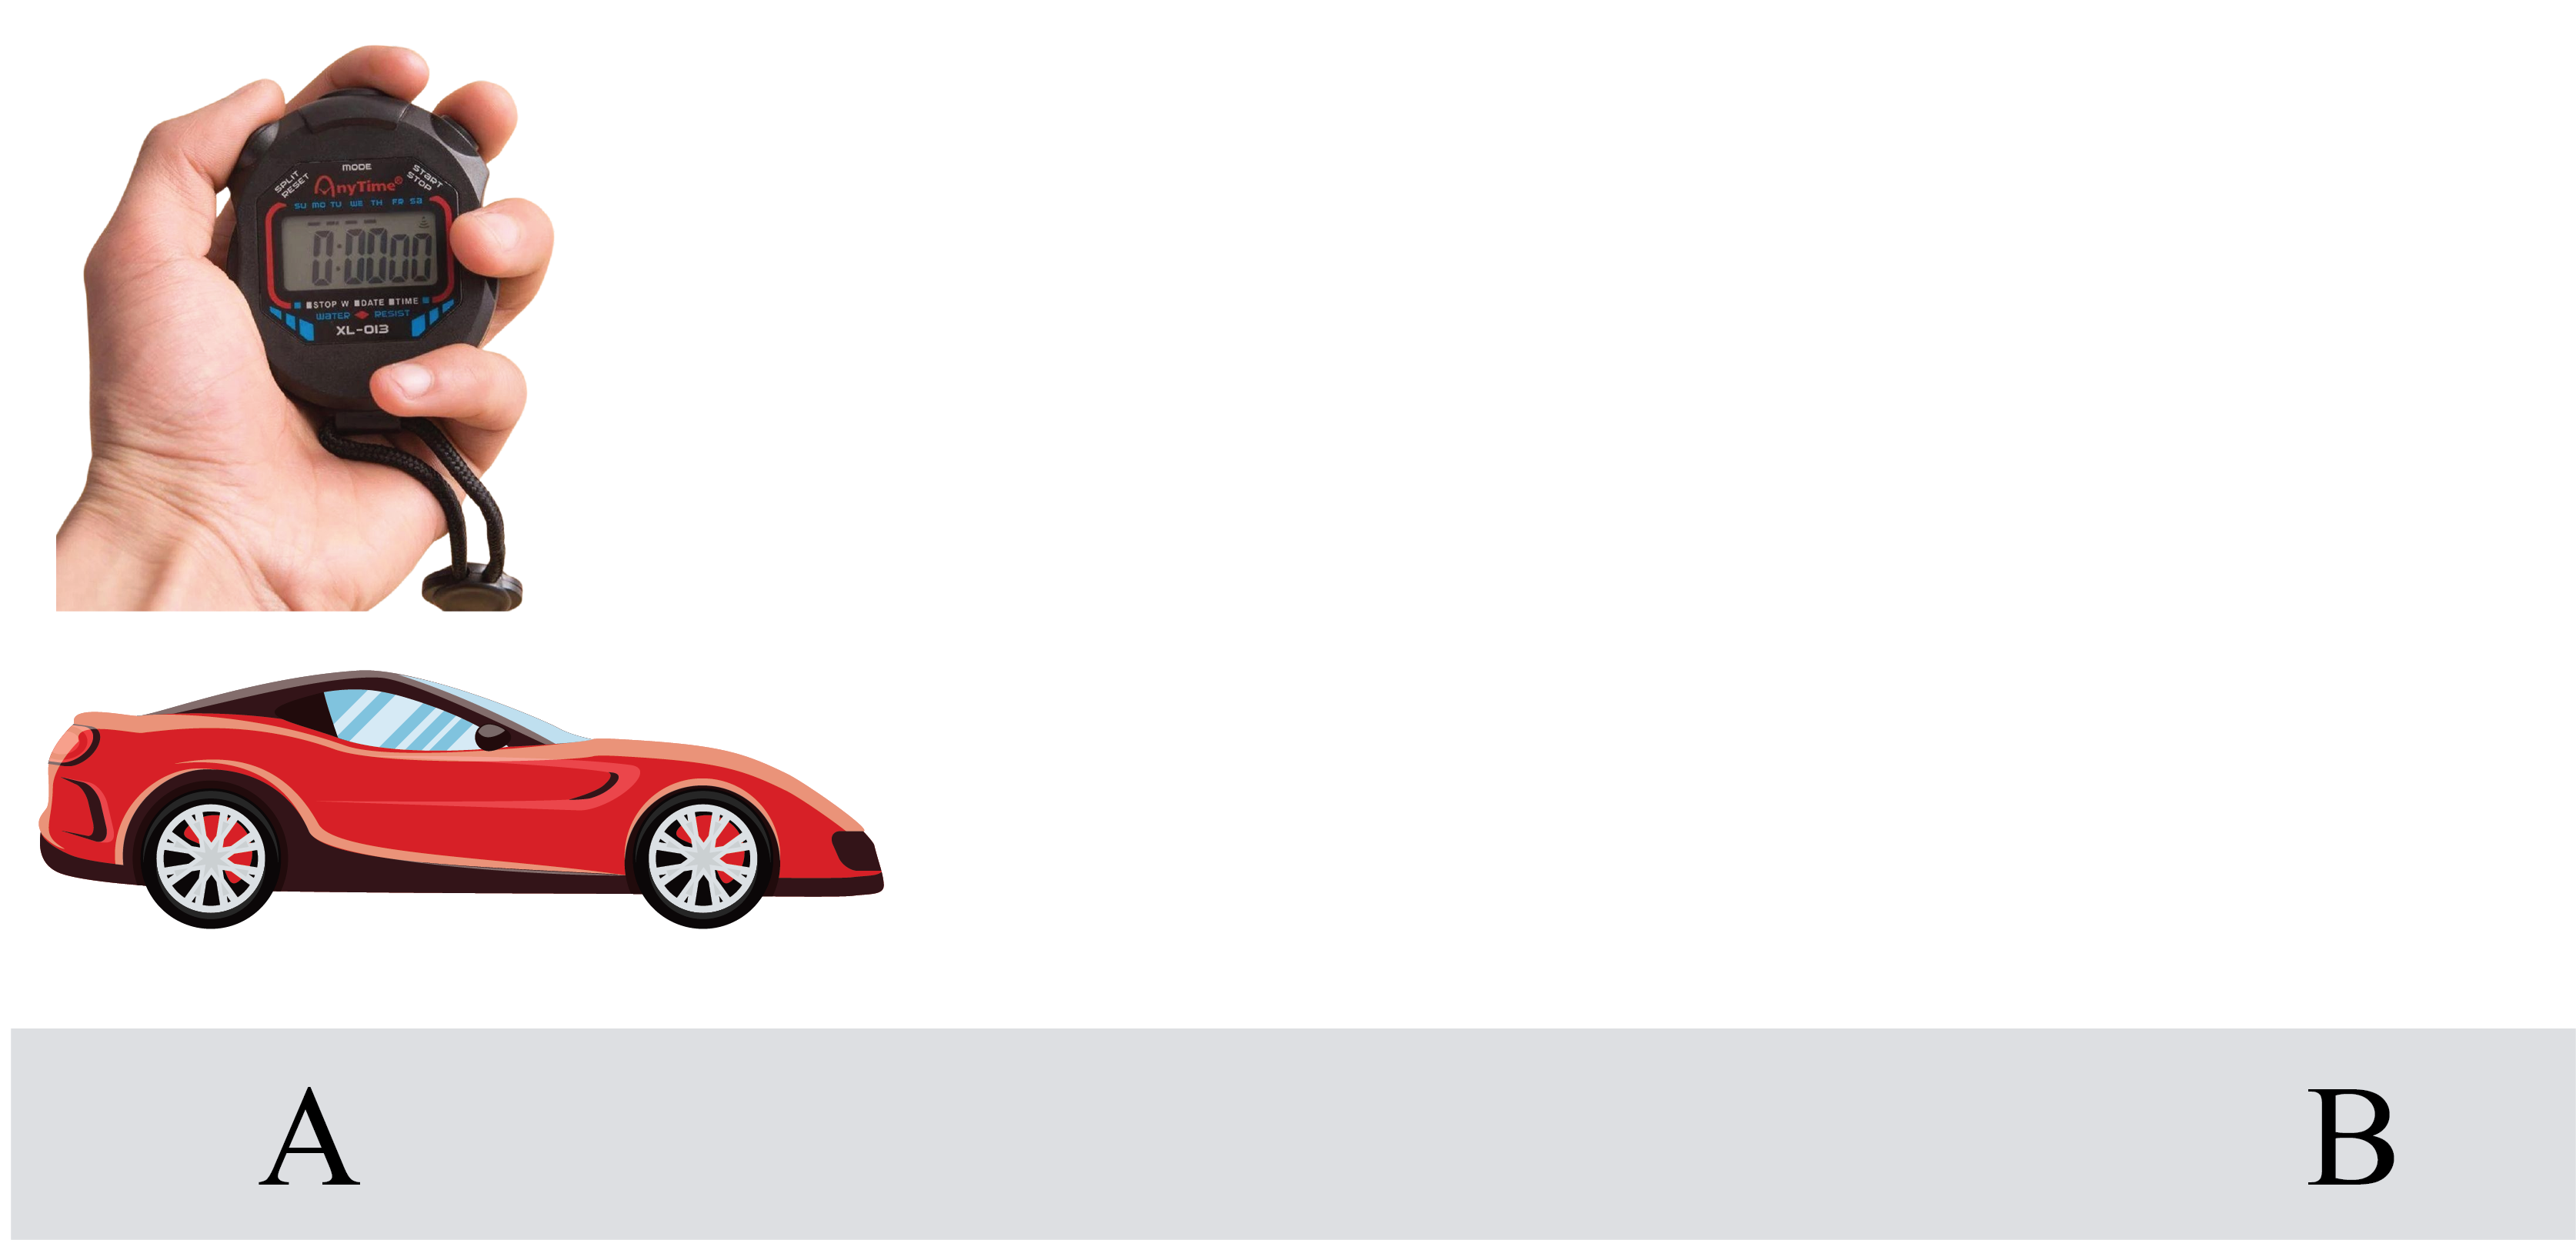
\includegraphics[width=0.6\linewidth]{figures/fig_p04_xe_do_choi.png}
\end{center}
\begin{enumerate}[a)]
    \item Nguyên nhân nào gây ra sự sai khác giữa các lần đo?
    \item Tính sai số tuyệt đối của phép đo $s, t$ và điền vào bảng. Lấy sai số dụng cụ bằng nửa độ chia nhỏ nhất của dụng cụ.
    \item Viết kết quả đo $s$ và $t$?
    \item Tính sai số tỉ đối của $s$ và $t$?
\end{enumerate}
\begin{center}
\renewcommand{\arraystretch}{1.15}
\begin{tabular}{|c|c|c|c|c|}
\hline
\textbf{Lần đo} & $s\text{ (mm)}$ & $\Delta s\text{ (mm)}$ & $t\text{ (s)}$ & $\Delta t\text{ (s)}$ \\
\hline
1 & 649 & & 3,49 & \\
2 & 651 & & 3,51 & \\
3 & 654 & & 3,54 & \\
4 & 653 & & 3,53 & \\
5 & 650 & & 3,50 & \\
\hline
\textbf{Trung bình} & & & & \\
\hline
\end{tabular}
\end{center}
\loigiai{
\begin{enumerate}[a)]
    \item \textbf{Nguyên nhân gây ra sự sai khác giữa các lần đo:}
    \begin{itemize}
        \item Do đặc điểm cấu tạo của dụng cụ đo.
        \item Do điều kiện làm thí nghiệm chưa thật ổn định (bề mặt trượt, điện áp pin thay đổi nhẹ).
        \item Do phản xạ và thao tác khi bấm đồng hồ hoặc quan sát vạch đo của người thực hiện.
    \end{itemize}
    \item \textbf{Bảng số liệu kết quả đo sau khi tính toán:}
    \begin{center}
    \renewcommand{\arraystretch}{1.15}
    \begin{tabular}{|c|c|c|c|c|}
    \hline
    \textbf{Lần đo} & $s\text{ (mm)}$ & $\Delta s\text{ (mm)}$ & $t\text{ (s)}$ & $\Delta t\text{ (s)}$ \\
    \hline
    1 & 649 & 2,4 & 3,49 & 0,024 \\
    2 & 651 & 0,4 & 3,51 & 0,004 \\
    3 & 654 & 2,6 & 3,54 & 0,026 \\
    4 & 653 & 1,6 & 3,53 & 0,016 \\
    5 & 650 & 1,4 & 3,50 & 0,014 \\
    \hline
    \textbf{Trung bình} & $\bar{s} = 651{,}4$ & $\overline{\Delta s} = 1{,}68$ & $\bar{t} = 3{,}514$ & $\overline{\Delta t} = 0{,}0168$ \\
    \hline
    \end{tabular}
    \end{center}
    Ta có:
    \[
    \bar{s} = \frac{649 + 651 + 654 + 653 + 650}{5} = 651{,}4\text{ mm}
    \]
    \[
    \overline{\Delta s} = \frac{|651{,}4 - 649| + |651{,}4 - 651| + |651{,}4 - 654| + |651{,}4 - 653| + |651{,}4 - 650|}{5} = 1{,}68\text{ mm}
    \]
    \[
    \bar{t} = \frac{3{,}49 + 3{,}51 + 3{,}54 + 3{,}53 + 3{,}50}{5} = 3{,}514\text{ s}
    \]
    \[
    \overline{\Delta t} = \frac{|3{,}514 - 3{,}49| + |3{,}514 - 3{,}51| + |3{,}514 - 3{,}54| + |3{,}514 - 3{,}53| + |3{,}514 - 3{,}50|}{5} = 0{,}0168\text{ s}
    \]
    \item \textbf{Viết kết quả đo:}
    \begin{itemize}
        \item Sai số dụng cụ: $\Delta s_{\text{dc}} = \frac{1}{2} = 0{,}5\text{ mm}$; $\Delta t_{\text{dc}} = \frac{0{,}01}{2} = 0{,}005\text{ s}$.
        \item Sai số tuyệt đối toàn phần:
        \[
        \Delta s = \overline{\Delta s} + \Delta s_{\text{dc}} = 1{,}68 + 0{,}5 = 2{,}18\text{ mm} \approx 2{,}2\text{ mm (hoặc } 2\text{ mm)}
        \]
        \[
        \Delta t = \overline{\Delta t} + \Delta t_{\text{dc}} = 0{,}0168 + 0{,}005 = 0{,}0218\text{ s} \approx 0{,}022\text{ s (hoặc } 0{,}02\text{ s)}
        \]
        \item Kết quả đo:
        \[
        s = \bar{s} \pm \Delta s = 651{,}4 \pm 2{,}2\text{ mm} \quad (\text{hoặc } 651 \pm 2\text{ mm})
        \]
        \[
        t = \bar{t} \pm \Delta t = 3{,}514 \pm 0{,}022\text{ s} \quad (\text{hoặc } 3{,}51 \pm 0{,}02\text{ s})
        \]
    \end{itemize}
    \item \textbf{Tính sai số tỉ đối:}
    \[
    \delta s = \frac{\Delta s}{\bar{s}} \cdot 100\% = \frac{2{,}2}{651{,}4} \cdot 100\% \approx 0{,}34\% \quad (\text{hoặc } \frac{2}{651} \cdot 100\% \approx 0{,}31\%)
    \]
    \[
    \delta t = \frac{\Delta t}{\bar{t}} \cdot 100\% = \frac{0{,}022}{3{,}514} \cdot 100\% \approx 0{,}63\% \quad (\text{hoặc } \frac{0{,}02}{3{,}51} \cdot 100\% \approx 0{,}57\%)
    \]
\end{enumerate}
}
\end{vd}

\begin{vd}
Đường kính của một viên bi trong 5 lần đo bằng $2{,}620\text{ cm}$; $2{,}625\text{ cm}$; $2{,}630\text{ cm}$; $2{,}628\text{ cm}$ và $2{,}626\text{ cm}$. Đường kính trung bình của viên bi là
\choice
{\True $2{,}6258\text{ cm}$}
{$2{,}6271\text{ cm}$}
{$2{,}6251\text{ cm}$}
{$2{,}6249\text{ cm}$}
\loigiai{
Giá trị trung bình của đường kính viên bi:
\[
\bar{d} = \frac{2{,}620 + 2{,}625 + 2{,}630 + 2{,}628 + 2{,}626}{5} = \frac{13{,}129}{5} = 2{,}6258\text{ cm}
\]
Chọn đáp án \textbf{A}.
}
\end{vd}

\begin{vd}
Kết quả ba lần đo quãng đường chuyển động của viên bi từ $A$ đến $B$ lần lượt là $0{,}048\text{ m}$; $0{,}050\text{ m}$; $0{,}050\text{ m}$, quãng đường trung bình là $0{,}049\text{ m}$. Khi đó sai số tuyệt đối của quãng đường chuyển động của viên bi qua ba lần đo có giá trị lần lượt là
\choice
{\True $0{,}001\text{ m}$; $0{,}001\text{ m}$; $0{,}001\text{ m}$}
{$-0{,}001\text{ m}$; $0{,}001\text{ m}$; $0{,}001\text{ m}$}
{$0{,}001\text{ m}$; $-0{,}001\text{ m}$; $-0{,}001\text{ m}$}
{$0{,}001\text{ m}$; $0{,}000\text{ m}$; $0{,}002\text{ m}$}
\loigiai{
Sai số tuyệt đối của mỗi lần đo là trị tuyệt đối hiệu số giữa giá trị trung bình và giá trị đo:
\begin{itemize}
    \item $\Delta s_1 = |\bar{s} - s_1| = |0{,}049 - 0{,}048| = 0{,}001\text{ m}$.
    \item $\Delta s_2 = |\bar{s} - s_2| = |0{,}049 - 0{,}050| = 0{,}001\text{ m}$.
    \item $\Delta s_3 = |\bar{s} - s_3| = |0{,}049 - 0{,}050| = 0{,}001\text{ m}$.
\end{itemize}
Chọn đáp án \textbf{A}.
}
\end{vd}

\begin{vd}
Để xác định thời gian đi của bạn A trên quãng đường $s$, người ta sử dụng đồng hồ bấm giây, thu được bảng số liệu dưới đây:
\begin{center}
\begin{tabular}{|c|c|c|c|}
\hline
\textbf{Lần đo} & 1 & 2 & 3 \\
\hline
\textbf{Thời gian (s)} & 35,20 & 36,15 & 35,75 \\
\hline
\end{tabular}
\end{center}
Coi tốc độ đi không đổi trong suốt quá trình chuyển động, sai số ngẫu nhiên trong phép đo này là bao nhiêu?
\choice
{$0{,}30\text{ s}$}
{$0{,}31\text{ s}$}
{$0{,}32\text{ s}$}
{\True $0{,}33\text{ s}$}
\loigiai{
Thời gian trung bình qua 3 lần đo:
\[
\bar{t} = \frac{35{,}20 + 36{,}15 + 35{,}75}{3} = \frac{107{,}10}{3} = 35{,}70\text{ s}
\]
Sai số tuyệt đối của từng lần đo:
\begin{itemize}
    \item $\Delta t_1 = |35{,}70 - 35{,}20| = 0{,}50\text{ s}$.
    \item $\Delta t_2 = |35{,}70 - 36{,}15| = 0{,}45\text{ s}$.
    \item $\Delta t_3 = |35{,}70 - 35{,}75| = 0{,}05\text{ s}$.
\end{itemize}
Sai số ngẫu nhiên (sai số tuyệt đối trung bình):
\[
\overline{\Delta t} = \frac{0{,}50 + 0{,}45 + 0{,}05}{3} = \frac{1{,}00}{3} \approx 0{,}33\text{ s}
\]
Chọn đáp án \textbf{D}.
}
\end{vd}

\begin{vd}
Dùng thước thẳng có giới hạn đo $20\text{ cm}$ và độ chia nhỏ nhất $0{,}5\text{ cm}$ để đo chiều dài chiếc bút máy. Lấy sai số dụng cụ bằng một nửa độ chia nhỏ nhất. Bỏ qua sai số ngẫu nhiên. Nếu chiếc bút có độ dài trung bình $15\text{ cm}$ thì phép đo này có sai số tuyệt đối và sai số tỉ đối là
\choice
{$0{,}5\text{ cm}$ và $2{,}5\%$}
{$0{,}5\text{ cm}$ và $1{,}7\%$}
{$0{,}25\text{ cm}$ và $2{,}5\%$}
{\True $0{,}25\text{ cm}$ và $1{,}7\%$}
\loigiai{
\begin{itemize}
    \item Sai số dụng cụ bằng một nửa ĐCNN: $\Delta \ell = \Delta \ell_{\text{dc}} = \frac{0{,}5}{2} = 0{,}25\text{ cm}$.
    \item Sai số tỉ đối của phép đo:
    \[
    \delta \ell = \frac{\Delta \ell}{\bar{\ell}} \cdot 100\% = \frac{0{,}25}{15} \cdot 100\% \approx 1{,}67\% \approx 1{,}7\%
    \]
\end{itemize}
Chọn đáp án \textbf{D}.
}
\end{vd}

\begin{vd}
Dùng thước kẹp có độ chia nhỏ nhất $0{,}1\text{ mm}$ để đo 5 lần đường kính $d$ của một trụ thép. Lấy sai số dụng cụ bằng một độ chia nhỏ nhất. Cho kết quả như trong bảng dưới. Hãy cho biết kết quả phép đo $d$.
\begin{center}
\begin{tabular}{|c|c|c|c|c|c|}
\hline
\textbf{Lần đo} & 1 & 2 & 3 & 4 & 5 \\
\hline
$d\text{ (mm)}$ & 30,0 & 30,1 & 30,0 & 30,1 & 30,1 \\
\hline
\end{tabular}
\end{center}
\choice
{\True $d = (30{,}06 \pm 0{,}15)\text{ mm}$}
{$d = (30{,}1 \pm 0{,}15)\text{ mm}$}
{$d = (30 \pm 0{,}1)\text{ mm}$}
{$d = (30{,}00 \pm 0{,}15)\text{ mm}$}
\loigiai{
\begin{itemize}
    \item Giá trị trung bình của đường kính:
    \[
    \bar{d} = \frac{30{,}0 \cdot 2 + 30{,}1 \cdot 3}{5} = \frac{150{,}3}{5} = 30{,}06\text{ mm}
    \]
    \item Sai số ngẫu nhiên:
    \[
    \overline{\Delta d} = \frac{|30{,}06 - 30{,}0|\cdot 2 + |30{,}06 - 30{,}1|\cdot 3}{5} = \frac{0{,}06 \cdot 2 + 0{,}04 \cdot 3}{5} = 0{,}048\text{ mm}
    \]
    \item Sai số dụng cụ bằng 1 ĐCNN: $\Delta d_{\text{dc}} = 0{,}1\text{ mm}$.
    \item Sai số tuyệt đối toàn phần: $\Delta d = \overline{\Delta d} + \Delta d_{\text{dc}} = 0{,}048 + 0{,}1 = 0{,}148\text{ mm} \approx 0{,}15\text{ mm}$.
    \item Kết quả phép đo: $d = (30{,}06 \pm 0{,}15)\text{ mm}$.
\end{itemize}
Chọn đáp án \textbf{A}.
}
\end{vd}

\begin{vd}
Một học sinh dùng đồng hồ bấm giây để đo chu kì chuyển động tròn của một vật bằng cách đo thời gian vật quay hết một vòng. Năm lần đo cho kết quả thời gian vật quay hết một vòng lần lượt là $2{,}00\text{ s}$; $2{,}05\text{ s}$; $2{,}00\text{ s}$; $2{,}05\text{ s}$; $2{,}05\text{ s}$. Thang chia nhỏ nhất của đồng hồ là $0{,}01\text{ s}$. Lấy sai số dụng cụ là một độ chia nhỏ nhất. Kết quả của phép đo chu kì được biểu diễn bằng
\choice
{$T = 2{,}030 \pm 0{,}02\text{ s}$}
{$T = 2{,}030 \pm 0{,}024\text{ s}$}
{\True $T = 2{,}030 \pm 0{,}034\text{ s}$}
{$T = 2{,}03 \pm 0{,}03\text{ s}$}
\loigiai{
\begin{itemize}
    \item Giá trị trung bình của chu kì:
    \[
    \bar{T} = \frac{2{,}00 + 2{,}05 + 2{,}00 + 2{,}05 + 2{,}05}{5} = 2{,}03\text{ s}
    \]
    \item Sai số dụng cụ bằng 1 ĐCNN: $\Delta T_{\text{dc}} = 0{,}01\text{ s}$.
    \item Sai số ngẫu nhiên:
    \[
    \overline{\Delta T} = \frac{|2{,}00 - 2{,}03| \cdot 2 + |2{,}05 - 2{,}03| \cdot 3}{5} = \frac{0{,}03 \cdot 2 + 0{,}02 \cdot 3}{5} = 0{,}024\text{ s}
    \]
    \item Sai số tuyệt đối toàn phần: $\Delta T = \overline{\Delta T} + \Delta T_{\text{dc}} = 0{,}024 + 0{,}01 = 0{,}034\text{ s}$.
    \item Kết quả phép đo: $T = (2{,}030 \pm 0{,}034)\text{ s}$.
\end{itemize}
Chọn đáp án \textbf{C}.
}
\end{vd}

\begin{vd}
Nhiệt độ đầu và nhiệt độ cuối của một lượng nước được ghi bởi một người quan sát trên nhiệt kế là $(42{,}4 \pm 0{,}2)^\circ\text{C}$ và $(80{,}6 \pm 0{,}3)^\circ\text{C}$. Bỏ qua sai số dụng cụ, nhiệt độ của nước đã tăng
\choice
{$(39{,}2 \pm 0{,}5)^\circ\text{C}$}
{$(38{,}2 \pm 0{,}1)^\circ\text{C}$}
{\True $(38{,}2 \pm 0{,}5)^\circ\text{C}$}
{$(39{,}2 \pm 0{,}1)^\circ\text{C}$}
\loigiai{
\begin{itemize}
    \item Độ tăng nhiệt độ trung bình: $\Delta \bar{t} = t_2 - t_1 = 80{,}6 - 42{,}4 = 38{,}2^\circ\text{C}$.
    \item Áp dụng quy tắc sai số của một hiệu, sai số tuyệt đối bằng tổng các sai số tuyệt đối:
    \[
    \Delta (\Delta t) = \Delta t_1 + \Delta t_2 = 0{,}2 + 0{,}3 = 0{,}5^\circ\text{C}
    \]
    \item Kết quả độ tăng nhiệt độ: $\Delta t = (38{,}2 \pm 0{,}5)^\circ\text{C}$.
\end{itemize}
Chọn đáp án \textbf{C}.
}
\end{vd}

\begin{vd}
Điện trở của một dây dẫn bằng kim loại được xác định theo định luật Ohm $R = \frac{U}{I}$. Trong một mạch điện, hiệu điện thế $U$ giữa hai đầu điện trở đo được là $U = (8 \pm 0{,}4)\text{ V}$ và cường độ dòng điện qua điện trở là $I = (4 \pm 0{,}2)\text{ A}$. Giá trị của điện trở cùng sai số tỉ đối bằng
\choice
{$(2 \pm 5\%)\,\Omega$}
{$(2 \pm 7\%)\,\Omega$}
{\True $(2 \pm 10\%)\,\Omega$}
{$(2 \pm 28\%)\,\Omega$}
\loigiai{
\begin{itemize}
    \item Giá trị trung bình của điện trở: $\bar{R} = \frac{\bar{U}}{\bar{I}} = \frac{8}{4} = 2\,\Omega$.
    \item Sai số tỉ đối của một thương bằng tổng các sai số tỉ đối:
    \[
    \delta R = \delta U + \delta I = \frac{\Delta U}{\bar{U}} \cdot 100\% + \frac{\Delta I}{\bar{I}} \cdot 100\% = \frac{0{,}4}{8}\cdot 100\% + \frac{0{,}2}{4}\cdot 100\% = 5\% + 5\% = 10\%
    \]
    \item Kết quả ghi: $R = (2 \pm 10\%)\,\Omega$.
\end{itemize}
Chọn đáp án \textbf{C}.
}
\end{vd}
\vspace{0.3cm}

\section*{C. ĐỀ LUYỆN TẬP SỐ 1}

\noindent\textbf{\large PHẦN I. Thí sinh trả lời từ câu 1 đến câu 18. Mỗi câu hỏi thí sinh chỉ chọn một phương án.}\par\vspace{0.2cm}
\begin{ex}
Phép đo của một đại lượng vật lí
\choice
{\True là phép so sánh nó với một đại lượng cùng loại được quy ước làm đơn vị.}
{là những sai sót gặp phải khi đo một đại lượng vật lí.}
{là sai sốgặp phải khi dụng cụđo một đại lượng vật lí.}
{là những công cụđo các đại lượng vật lí như thước, cân...vv.}
\loigiai{
Chọn đáp án \textbf{A}
. . . . . . . . . . . . . . . . . . . . . . . . . . . . . . . . . . . . . . . . . . . . . . . . . . . . . . . . . . . . . . . . . . . . .
}
\end{ex}

\begin{ex}
Trong đơn vịSI, đơn vịnào là đơn vịdẫn xuất?
\choice
{mét (m).}
{giây (s).}
{mol (mol).}
{\True mét trên giây (m/s).}
\loigiai{
Chọn đáp án \textbf{D} . . . . . . . . . . . . . . . . . . . . . . . . . . . . . . . . . . . . . . . . . . . . . . . . . . . . . . . . . . . . . . . . . . . . .
}
\end{ex}

\begin{ex}
Có mấy cách đểđo các đại lượng vật lí?
\choice
{1.}
{\True 2.}
{3.}
{4.}
\loigiai{
Chọn đáp án \textbf{B}
. . . . . . . . . . . . . . . . . . . . . . . . . . . . . . . . . . . . . . . . . . . . . . . . . . . . . . . . . . . . . . . . . . . . .
}
\end{ex}

\begin{ex}
Trong các phép đo dưới đây, đâu là phép đo trực tiếp?
(1) Dùng thước đo chiều cao.
(2) Dùng cân đo cân nặng.
(3) Dùng cân và ca đong đo khối lượng riêng của nước.
(4) Dùng đồng hồvà cột cây sốđo tốc độcủa người lái xe.
\choice
{\True (1), (2).}
{(2), (4).}
{(1), (2), (4).}
{(2), (3), (4).}
\loigiai{
Chọn đáp án \textbf{A}
. . . . . . . . . . . . . . . . . . . . . . . . . . . . . . . . . . . . . . . . . . . . . . . . . . . . . . . . . . . . . . . . . . . . .
}
\end{ex}

\begin{ex}
Một học sinh dùng thước đo chiều dài có độchia nhỏnhất là 1 milimet, đồng
hồbấm giây đểđo quãng đường, thời gian và tốc độchuyển động của chiếc xe đồchơi.
Phát biểu nào sau đây là sai?
\choice
{\True Đo tốc độlà phép đo trực tiếp.}
{Đo thời gian là phép đo trực tiếp.}
{Sai sốdụng cụcủa thước đo chiều dài là 0,5 mm.}
{Đo quãng đường là phép đo trực tiếp.}
\loigiai{
Chọn đáp án \textbf{A}
. . . . . . . . . . . . . . . . . . . . . . . . . . . . . . . . . . . . . . . . . . . . . . . . . . . . . . . . . . . . . . . . . . . . .
}
\end{ex}

\begin{ex}
Kết quảsai sốtuyệt đối của một phép đo là 0,0809. Sốchữsốcó nghĩa là
\choice
{4.}
{2.}
{1.}
{\True 3.}
\loigiai{
Số0,0809 có 3 chữsốcó nghĩa.
Chọn đáp án \textbf{D} . . . . . . . . . . . . . . . . . . . . . . . . . . . . . . . . . . . . . . . . . . . . . . . . . . . . . . . . . . . . . . . . . . . . .
}
\end{ex}

\begin{ex}
Kết quảsai sốtuyệt đối của một phép đo là 0,4009. Sốchữsốcó nghĩa là
\choice
{\True 4.}
{1.}
{2.}
{3.}
\loigiai{
Số0,4009 có 4 chữsốcó nghĩa.
Chọn đáp án \textbf{A}
. . . . . . . . . . . . . . . . . . . . . . . . . . . . . . . . . . . . . . . . . . . . . . . . . . . . . . . . . . . . . . . . . . . . .
}
\end{ex}

\begin{ex}
Sai sốhệthống là
\choice
{\True sai sốcó tính quy luật và được lặp lại ởtất cảcác lần đo.}
{sai sốtừnhững yếu tốngẫu nhiên bên ngoài.}
{sai sốxuất phát từsai sót, phản xạcủa người làm thí nghiệm.}
{sai sốtuyệt đối.}
\loigiai{
Chọn đáp án \textbf{A}
. . . . . . . . . . . . . . . . . . . . . . . . . . . . . . . . . . . . . . . . . . . . . . . . . . . . . . . . . . . . . . . . . . . . .
}
\end{ex}

\begin{ex}
$\Delta$Ai =A-$\Delta$Ailà công thức tính
\choice
{\True sai sốtuyệt đối ứng với mỗi lần đo.}
{sai sốtuyệt đối trung bình của n lần đo.}
{giá trịtrung bình của đại lượng cần đo khi tiến hành phép đo nhiều lần.}
{sai sốtuyệt đối của phép đo.}
\loigiai{
Chọn đáp án \textbf{A}
. . . . . . . . . . . . . . . . . . . . . . . . . . . . . . . . . . . . . . . . . . . . . . . . . . . . . . . . . . . . . . . . . . . . .
}
\end{ex}

\begin{ex}
Điều nào sau đây không đúng khi nói vềnguyên nhân gây ra sai sốngẫu
nhiên trong quá trình đo một đại lượng vật lí?
\choice
{Thao tác đo không chuẩn.}
{\True Dụng cụđo không chuẩn.}
{Điều kiện làm thí nghiệm không ổn định.}
{Mắt người đọc không chuẩn.}
\loigiai{
Chọn đáp án \textbf{B}
. . . . . . . . . . . . . . . . . . . . . . . . . . . . . . . . . . . . . . . . . . . . . . . . . . . . . . . . . . . . . . . . . . . . .
}
\end{ex}

\begin{ex}
Sai sốtỉđối của phép đo là
\choice
{$\delta$x = $\Delta$x x .100\%.}
{\True $\delta$x = $\Delta$x x .100\%.}
{$\delta$x = $\Delta$xdc x .100\%.}
{$\delta$x = $\Delta$x x .100\%.}
\loigiai{
Chọn đáp án \textbf{B}
. . . . . . . . . . . . . . . . . . . . . . . . . . . . . . . . . . . . . . . . . . . . . . . . . . . . . . . . . . . . . . . . . . . . .
}
\end{ex}

\begin{ex}
Một phép đo đại lượng vật lí A thu được giá trịtrung bình là A, sai sốcủa
phép đo là $\Delta$A. Cách ghi đúng kết quảđo A là
\choice
{A = A+$\Delta$A.}
{A = A-$\Delta$A.}
{A = A$\pm$$\Delta$A.}
{\True A = A$\pm$$\Delta$A.}
\loigiai{
Chọn đáp án \textbf{D} . . . . . . . . . . . . . . . . . . . . . . . . . . . . . . . . . . . . . . . . . . . . . . . . . . . . . . . . . . . . . . . . . . . . .
}
\end{ex}

\begin{ex}
Sai sốcủa một tích A = B.C trong phép đo gián tiếp được xác định bởi công
thức?
\choice
{\True $\delta$A = $\delta$B+$\delta$C.}
{$\Delta$A = $\Delta$B+$\Delta$C.}
{$\delta$A = $\Delta$B+$\Delta$C.}
{$\Delta$A = $\delta$B+$\delta$C.}
\loigiai{
Chọn đáp án \textbf{A}
. . . . . . . . . . . . . . . . . . . . . . . . . . . . . . . . . . . . . . . . . . . . . . . . . . . . . . . . . . . . . . . . . . . . .
}
\end{ex}

\begin{ex}
Khi đo chiều dài L của chiếc bàn học, một học sinh viết được kết quảlà
L = 118$\pm$2 cm. Giá trịtrung bình của L là
\choice
{2 cm.}
{120 cm.}
{\True 118 cm.}
{116 cm.}
\loigiai{
Chọn đáp án \textbf{C}
. . . . . . . . . . . . . . . . . . . . . . . . . . . . . . . . . . . . . . . . . . . . . . . . . . . . . . . . . . . . . . . . . . . . .
}
\end{ex}

\begin{ex}
Bạn Bình tiến hành cân một viên bi nhỏnhiều lần và tính được kết quảkhối
lượng của viên bi như sau: m = 6,03$\pm$0,04 g. Sai sốtuyệt đối của phép đo khối lượng viên
bi là
\choice
{\True 0,04 g.}
{6,03 g.}
{0,7\%.}
{0,6\%.}
\loigiai{
Chọn đáp án \textbf{A}
. . . . . . . . . . . . . . . . . . . . . . . . . . . . . . . . . . . . . . . . . . . . . . . . . . . . . . . . . . . . . . . . . . . . .
}
\end{ex}

\begin{ex}
Một người dùng thước đo có độchia nhỏnhất 1 cm đểđo chiều cao một người
khác trong ba lần được là 160 cm; 161 cm; 162 cm. Lấy sai sốdụng cụbằng một độchia
nhỏnhất. Sai sốtỉđối của phép đo là
\choice
{0,23\%.}
{7,2\%.}
{0,41\%.}
{\True 1,04\%.}
\loigiai{
\item L = 161 cm.
\item $\Delta$A = 1+0+1
3
= 2
3

\item $\Delta$A = $\Delta$A+$\Delta$ADC = 2
3 +1 = 5
3 cm.
\item $\delta$A = $\Delta$A
A
=
5
3
161 $\approx$1,04\%
Chọn đáp án \textbf{D} . . . . . . . . . . . . . . . . . . . . . . . . . . . . . . . . . . . . . . . . . . . . . . . . . . . . . . . . . . . . . . . . . . . . .
}
\end{ex}

\begin{ex}
Dùng một cái cân có độchia nhỏnhất là 0,1 kg đểcân 5 lần khối lượng của
một bao gạo đều bằng 20 kg. Lấy sai sốdụng cụbằng một độchia nhỏnhất. Kết quảcủa
phép cân này là
\choice
{20$\pm$0,1 kg.}
{20,0$\pm$0,2 kg.}
{20,00$\pm$0,1 kg.}
{\True 20,0$\pm$0,1 kg.}
\loigiai{
\item Do 5 lần cân đều cho kết quả20 kg nên sai sốngẫu nhiên $\Delta$m = 0.
\item Sai sốcủa phép cân bằng sai sốdụng cụ: $\Delta$m = $\Delta$mdc = 0,1 kg.
\item Kết quảcủa phép cân: 20,0$\pm$0,1 (kg).
Chọn đáp án \textbf{D} . . . . . . . . . . . . . . . . . . . . . . . . . . . . . . . . . . . . . . . . . . . . . . . . . . . . . . . . . . . . . . . . . . . . .
}
\end{ex}

\begin{ex}
Đểđo dòng điện một chiều có cường độ25 mA bằng đồng hồvạn năng, người
ta tiến hành các bước:
(1) Kết nối que đo màu đỏcủa đồng hồvềphía cực (+) và que đo màu
đen vềphía cực (-) theo chiều dòng điện trong mạch thí nghiệm.
Mắc đồng hồnối tiếp với mạch thí nghiệm.
(2) Đọc kết quảđo hiện trên đồng hồ.
(3) Tắt nguồn điện của các mạch thí nghiệm.
(4) Cắm que đo màu đen vào đầu COM và que đỏvào dấu (+).
(5) Đặt chuyển mạch của đồng hồởthang DCmA.
(6) Bật điện cho mạch thí nghiệm.
Thứtựcác bước tiến hành đúng là
\choice
{\True (4); (5); (3); (1); (6); (2).}
{(6); (5); (4); (3); (1); (2).}
{(1); (2); (3); (4); (5); (6).}
{(3); (1); (6); (5); (4); (2).}
\loigiai{
Chọn đáp án \textbf{A}
. . . . . . . . . . . . . . . . . . . . . . . . . . . . . . . . . . . . . . . . . . . . . . . . . . . . . . . . . . . . . . . . . . . . .
}
\end{ex}

\vspace{0.4cm}\noindent\textbf{\large PHẦN II. Thí sinh trả lời từ câu 1 đến câu 4. Trong mỗi ý a), b), c), d) ở mỗi câu, thí sinh chọn đúng hoặc sai.}\par\vspace{0.2cm}
\begin{ex}
Nếu một đại lượng được đo trực tiếp.
\choiceTF[t]
{\True Giá trịtrung bình của đại lượng cần đo khi tiến hành phép đo nhiều lần được xác định bằng công thức A = A1 +A2 +...+An n .}
{\True Sai sốdụng cụthường được lấy bằng một nửa độchia nhỏnhất trên dụng cụ.}
{Sai sốtỉđối của phép đo càng lớn thì phép đo càng chính xác.}
{Sai sốcủa phép đo chiều dài một đại lượng có kết quảlà 0,03 cm. Sốchữsố có nghĩa trong kết quảcủa phép đo này là 3.}
\loigiai{
a) Đ
b) Đ
c) S
d) S
Chọn đáp án a đúng
b đúng
c sai
d sai . . . . . . . . . . . . . . . . . . . . . . . . . . . . . . . . . . . . . . .
}
\end{ex}

\begin{ex}
Hình vẽ thể hiện nhiệt kế đo nhiệt độ $t_1(^\circ\text{C})$ và $t_2(^\circ\text{C})$ của một dung dịch trước và sau khi đun:
\begin{center}
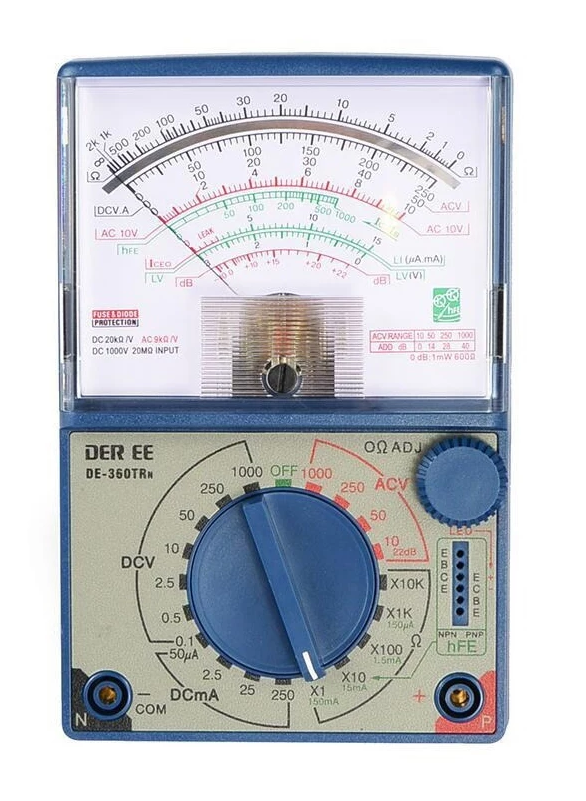
\includegraphics[width=0.4\linewidth]{figures/fig_p11_nhiet_ke.png}
\end{center}
\choiceTF[t]
{\True Giá trị đo nhiệt độ $t_1(^\circ\text{C})$ của dung dịch trước khi đun là $t_1 = 24{,}0 \pm 0{,}5^\circ\text{C}$.}
{Giá trị đo nhiệt độ $t_2(^\circ\text{C})$ của dung dịch sau khi đun là $t_2 = 68{,}0 \pm 0{,}05^\circ\text{C}$.}
{Sai số tuyệt đối của phép đo nhiệt độ này là $1{,}5^\circ\text{C}$.}
{\True Kết quả độ tăng nhiệt độ của dung dịch là: $\Delta t = 44{,}0 \pm 1{,}0^\circ\text{C}$.}
\loigiai{
a) Đ
b) S
c) S
d) Đ
Chọn đáp án a đúng
b sai
c sai
d đúng . . . . . . . . . . . . . . . . . . . . . . . . . . . . . . . . . . . . . . .
}
\end{ex}

\begin{ex}
Hai người cùng đo chiều dài của cánh cửa sổ, kết quảthu được như sau:
\item Người thứnhất: d = 120$\pm$1 cm
\item Người thứhai: d = 120$\pm$2 cm
\choiceTF[t]
{\True Sai sốtỉđối được xác định bằng tỉsốgiữa hai sốtuyệt đối và giá trịtrung bình của chiều dài cánh cửa số: $\delta$d = $\Delta$d d .100\%.}
{Sai sốtỉđối của phép đo của người thứnhất là 8,3\%.}
{\True Sai sốtỉđối của phép đo của người thứhai là 1,67\%.}
{Người thứhai đo chính xác hơn người thứnhất vì sai sốtỉđối của người thứ nhất lớn hơn.}
\loigiai{
a) Đ
b) S
c) Đ
d) S
Chọn đáp án a đúng
b sai
c đúng
d sai . . . . . . . . . . . . . . . . . . . . . . . . . . . . . . . . . . . . . . .
}
\end{ex}

\begin{ex}
Một học sinh đo tốc độtrung bình của viên bi được giá trịv = (2,50$\pm$0,04) m/s.
\choiceTF[t]
{\True Giá trịtrung bình của tốc độcủa viên bi là 2,54 m/s.}
{\True Sai sốtuyệt đối của phép đo tốc độviên bi là 0,04.}
{\True Sai sốtỉđối của phép đo là 1,6\%.}
{Nếu sai sốtỉđối của thời gian là 1\% thì sai sốtỉđối của quãng đường là 1,6\%.}
\loigiai{
a) Đ
b) Đ
c) Đ
d) S
Chọn đáp án a đúng
b đúng
c đúng
d sai
. . . . . . . . . . . . . . . . . . . . . . . . . . . . . . . . . . . .
}
\end{ex}

\vspace{0.4cm}\noindent\textbf{\large PHẦN III. Thí sinh trả lời từ câu 1 đến câu 6. Câu hỏi trắc nghiệm trả lời ngắn.}\par\vspace{0.2cm}
\begin{ex}
Lấy sai số dụng cụ bằng nửa độ chia nhỏ nhất. Sai số dụng cụ của cây bút chì trong trường hợp dưới đây là bao nhiêu $\text{cm}$?
\begin{center}
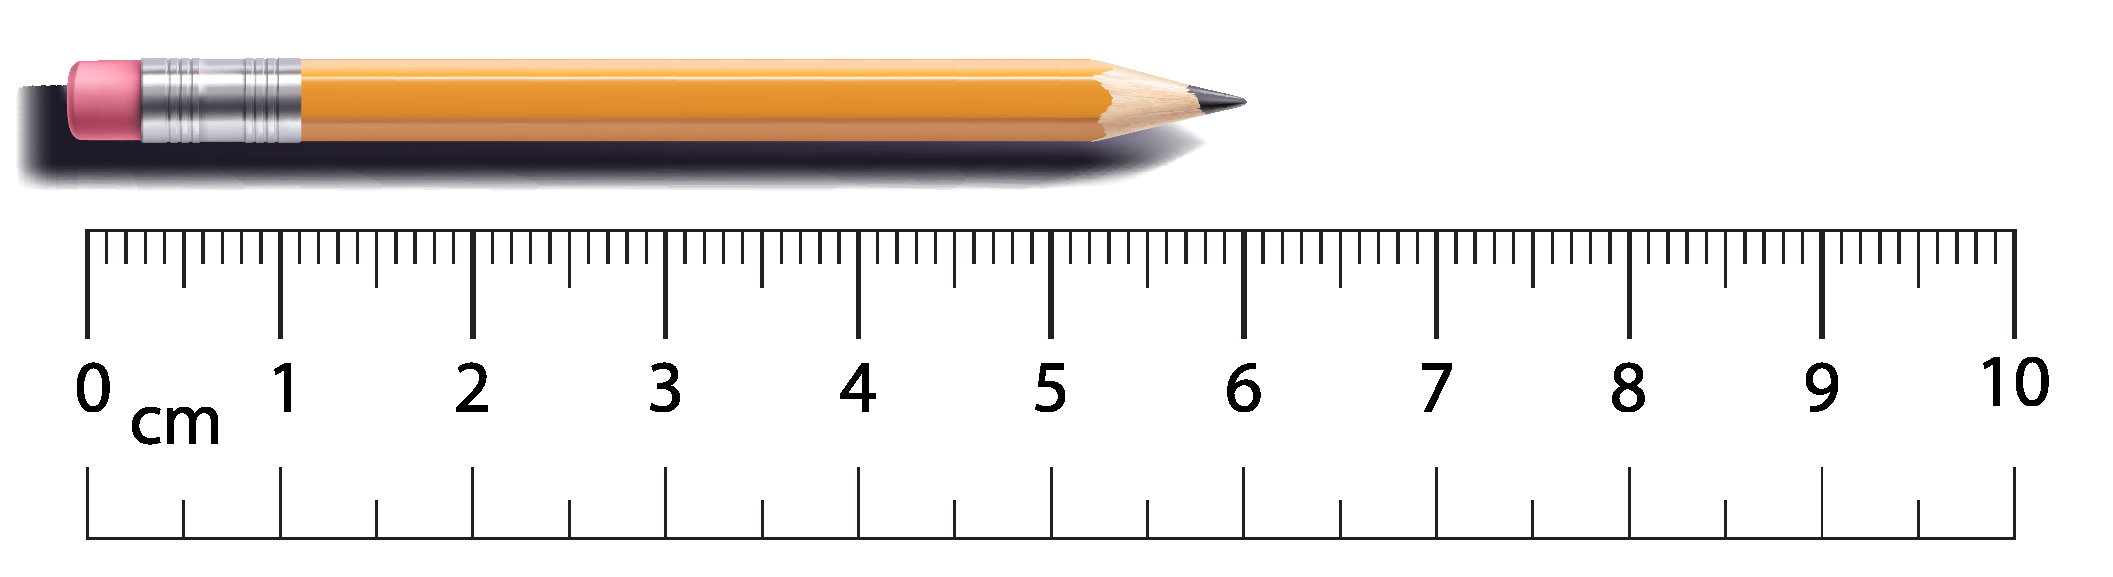
\includegraphics[width=0.75\linewidth]{figures/fig_p13_thuoc_kep.png}
\end{center}
\shortans{0,05}
\loigiai{
Đáp án: \textbf{0,05} . . . . . . . . . . . . . . . . . . . . . . . . . . . . . . . . . . . . . . . . . . . . . . . . . . . . . . . . . . . . . . . . . . . . . . .
}
\end{ex}

\begin{ex}
Đường kính của một quảbóng bằng (5,0$\pm$0,2) cm. Sai sốtỉđối của phép đo thể
tích quảbóng có giá trịlà x\%. Tìm x.
\shortans{12}
\loigiai{
\item Thểtích quảbóng là V = 4
3$\pi$R3
\item Sai sốtỉđối của phép đo thểtích:
$\delta$(V) = $\Delta$V
V 100\% = 3$\Delta$R
R .100\% = 3$\Delta$d
d .100\% = 30,2
5,0100\% = 12\%
Đáp án: \textbf{12} . . . . . . . . . . . . . . . . . . . . . . . . . . . . . . . . . . . . . . . . . . . . . . . . . . . . . . . . . . . . . . . . . . . . . . . . .
}
\end{ex}

\begin{ex}
Đểtính gia tốc rơi tựdo g, người ta có thểdùng công thức tính chu kì của một
con lắc đơn gồm một vật nặng có kích thước nhỏtreo vào một dây nhẹ, không co giãn:
$T = 2\pi \sqrt{\frac{\ell}{g}}$, trong đó, T là thời gian đểvật nặng thực hiện một dao động và $\ell$là chiều
dài sợi dây. Trong thí nghiệm với con lắc đơn, người ta đo được: $\ell$= 0,350$\pm$0,005 (m) và
T = 1,18$\pm$0,02 (s). Sai sốtuyệt đối của phép đo này là bao nhiêu m/s2 (làm tròn kết quả
đến chữsốhàng phần mười)?
\shortans{0,5}
\loigiai{
Đáp án: \textbf{0,5} . . . . . . . . . . . . . . . . . . . . . . . . . . . . . . . . . . . . . . . . . . . . . . . . . . . . . . . . . . . . . . . . . . . . . . . .
}
\end{ex}

\begin{ex}
Dùng thước thẳng có giới hạn đo là 20 cm và độchia nhỏnhất là 0,5 cm đểđo
chiều dài chiếc bút máy. Nếu chiếc bút có độdài cỡ15 cm thì phép đo này sai sốtỉđối là
bao nhiêu \% (làm tròn kết quảđến chữsốhàng phần trăm)?
\shortans{1,67}
\loigiai{
Đáp án: \textbf{1,67} . . . . . . . . . . . . . . . . . . . . . . . . . . . . . . . . . . . . . . . . . . . . . . . . . . . . . . . . . . . . . . . . . . . . . . .
}
\end{ex}

\begin{ex}
Kết quảđo đường kính của một đường tròn là d = (40,1$\pm$0,2) cm. Sai sốtuyệt
đối của phép đo diện tích này bằng x.103 cm2. Tìm x (làm tròn kết quảđến chữsốhàng
phần trăm).
\shortans{0,01}
\loigiai{
Đáp án: \textbf{0,01} . . . . . . . . . . . . . . . . . . . . . . . . . . . . . . . . . . . . . . . . . . . . . . . . . . . . . . . . . . . . . . . . . . . . . . .
}
\end{ex}

\begin{ex}
Kết quảcủa phép đo chiều dài và chiều rộng của một hình chữnhật lần lượt là
a = 85,0$\pm$0,2 (cm) và b = 29,5$\pm$0,2 (cm). Sai sốtỉđối của phép đo diện tích hình chữnhật
là bao nhiêu \% (làm tròn kết quảđến chữsốhàng phần mười)?
\shortans{0,9}
\loigiai{
Đáp án: \textbf{0,9} . . . . . . . . . . . . . . . . . . . . . . . . . . . . . . . . . . . . . . . . . . . . . . . . . . . . . . . . . . . . . . . . . . . . . . . .
}
\end{ex}

\section*{D. ĐỀ LUYỆN TẬP SỐ 2}

\noindent\textbf{\large PHẦN I. Thí sinh trả lời từ câu 1 đến câu 18. Mỗi câu hỏi thí sinh chỉ chọn một phương án.}\par\vspace{0.2cm}
\begin{ex}
Đại lượng nào là đại lượng cơ bản của hệSI?
\choice
{\True Cường độdòng điện.}
{Hiệu điện thế.}
{Công suất.}
{Điện trở.}
\loigiai{
Chọn đáp án \textbf{A}
. . . . . . . . . . . . . . . . . . . . . . . . . . . . . . . . . . . . . . . . . . . . . . . . . . . . . . . . . . . . . . . . . . . . .
}
\end{ex}

\begin{ex}
Đơn vịđo thời gian trong hệthống đo lường chính thức ởnước ta hiện nay là
\choice
{tuần.}
{ngày.}
{giờ.}
{\True giây.}
\loigiai{
Chọn đáp án \textbf{D} . . . . . . . . . . . . . . . . . . . . . . . . . . . . . . . . . . . . . . . . . . . . . . . . . . . . . . . . . . . . . . . . . . . . .
}
\end{ex}

\begin{ex}
Phép đo trực tiếp của một đại lượng vật lí là phép
\choice
{\True so sánh trực tiếp qua dụng cụđo.}
{so sánh gián tiếp qua dụng cụđo.}
{so sánh không thông qua dụng cụđo.}
{đo đại lượng thứnhất rồi suy ra đại lượng cần đo thông qua công thức.}
\loigiai{
Chọn đáp án \textbf{A}
. . . . . . . . . . . . . . . . . . . . . . . . . . . . . . . . . . . . . . . . . . . . . . . . . . . . . . . . . . . . . . . . . . . . .
}
\end{ex}

\begin{ex}
Phép đo nào sau đây không thểthực hiện đo trực tiếp?
\choice
{Đo thời gian.}
{Đo khối lượng.}
{\True Đo khối lượng riêng.}
{Đo chiều dài.}
\loigiai{
Chọn đáp án \textbf{C}
. . . . . . . . . . . . . . . . . . . . . . . . . . . . . . . . . . . . . . . . . . . . . . . . . . . . . . . . . . . . . . . . . . . . .
}
\end{ex}

\begin{ex}
Thiết bịnào sau đây dùng đểđo điện năng tiêu thụtrong các hộgia đình?
\choice
{Vôn kế.}
{Ampe kế.}
{\True Công tơ điện.}
{Nhiệt kế.}
\loigiai{
Chọn đáp án \textbf{C}
. . . . . . . . . . . . . . . . . . . . . . . . . . . . . . . . . . . . . . . . . . . . . . . . . . . . . . . . . . . . . . . . . . . . .
}
\end{ex}

\begin{ex}
Kết quảsai sốtuyệt đối của một phép đo là 6,07. Sốchữsốcó nghĩa là
\choice
{4.}
{2.}
{\True 3.}
{1.}
\loigiai{
Số6,07 có 3 chữsốcó nghĩa.
Chọn đáp án \textbf{C}
. . . . . . . . . . . . . . . . . . . . . . . . . . . . . . . . . . . . . . . . . . . . . . . . . . . . . . . . . . . . . . . . . . . . .
}
\end{ex}

\begin{ex}
Sai sốphép đo bao gồm
\choice
{sai sốngẫu nhiên và sai sốđơn vị.}
{\True sai sốngẫu nhiên và sai sốhệthống.}
{sai sốhệthống và sai sốđơn vị.}
{sai sốđơn vịvà sai sốdụng cụ.}
\loigiai{
Chọn đáp án \textbf{B}
. . . . . . . . . . . . . . . . . . . . . . . . . . . . . . . . . . . . . . . . . . . . . . . . . . . . . . . . . . . . . . . . . . . . .
}
\end{ex}

\begin{ex}
Sai sốhệthống có thểđược hạn chếbằng cách thường xuyên
\choice
{hiệu chỉnh dụng cụđo, vệsinh dụng cụđo.}
{đeo kính lúp khi đo, vệsinh dụng cụđo.}
{\True hiệu chỉnh dụng cụđo, sửdụng thiết bịđo có độchính xác cao.}
{sửdụng thiết bịđo có độchính xác cao, đeo kính lúp khi đo.}
\loigiai{
Chọn đáp án \textbf{C}
. . . . . . . . . . . . . . . . . . . . . . . . . . . . . . . . . . . . . . . . . . . . . . . . . . . . . . . . . . . . . . . . . . . . .
}
\end{ex}

\begin{ex}
Khi đo n lần cùng một đại lượng A, ta nhận được các giá trịkhác nhau: A1, A2,
..., An. Giá trịtrung bình của A là A. Sai sốtuyệt đối ứng với lần đo thứ4 được tính bằng
công thức nào sau đây?
\choice
{\True $\Delta$A4 =A-A4.}
{$\Delta$A4 = A-A4 2 .}
{$\Delta$A4 = A+A4 2 .}
{$\Delta$A4 =A+A4.}
\loigiai{
Chọn đáp án \textbf{A}
. . . . . . . . . . . . . . . . . . . . . . . . . . . . . . . . . . . . . . . . . . . . . . . . . . . . . . . . . . . . . . . . . . . . .
}
\end{ex}

\begin{ex}
Sai sốngẫu nhiên có thểđược hạn chếbằng cách
\choice
{\True thực hiện phép đo nhiều lần và lấy giá trịtrung bình đểhạn chếsựphân tán của sốliệu đo.}
{hiệu chỉnh dụng cụđo, sửdụng thiết bịđo có độchính xác cao.}
{hiệu chỉnh dụng cụđo, thực hiện phép đo nhiều lần.}
{thực hiện phép đo nhiều lần, sửdụng thiết bịđo có độchính xác cao.}
\loigiai{
Chọn đáp án \textbf{A}
. . . . . . . . . . . . . . . . . . . . . . . . . . . . . . . . . . . . . . . . . . . . . . . . . . . . . . . . . . . . . . . . . . . . .
}
\end{ex}

\begin{ex}
Sai sốtỉđối của phép đo là
\choice
{tỉsốgiữa sai sốtuyệt đối và sai sốngẫu nhiên.}
{tỉsốgiữa sai ngẫu nhiên và sai sốhệthống.}
{\True tỉsốgiữa sai sốtuyệt đối và giá trịtrung bình của đại lượng cần đo.}
{tỉsốgiữa sai sốngẫu nhiên và sai sốtuyệt đối.}
\loigiai{
Chọn đáp án \textbf{C}
. . . . . . . . . . . . . . . . . . . . . . . . . . . . . . . . . . . . . . . . . . . . . . . . . . . . . . . . . . . . . . . . . . . . .
}
\end{ex}

\begin{ex}
Khi đo nhiều lần thời gian chuyển động của một viên bi trên mặt phẳng
nghiêng mà thu được nhiều giá trịkhác nhau, thì giá trịnào sau đây được lấy làm kết
quảcủa phép đo?
\choice
{Giá trịtrung bình của giá trịlớn nhất và giá trịnhỏnhất.}
{\True Giá trịtrung bình của tất cảcác giá trịđo được.}
{Giá trịcủa lần đo cuối cùng.}
{Giá trịđược lặp lại nhiều lần nhất.}
\loigiai{
Chọn đáp án \textbf{B}
. . . . . . . . . . . . . . . . . . . . . . . . . . . . . . . . . . . . . . . . . . . . . . . . . . . . . . . . . . . . . . . . . . . . .
}
\end{ex}

\begin{ex}
Trong bài thực hành đo tốc độcủa vật chuyển động. Đểđo tốc độtrung bình
của vật ta sửdụng biểu thức v = s
t. Khi đó
\choice
{$\Delta$v = $\Delta$s-$\Delta$t.}
{$\Delta$v = $\Delta$s+$\Delta$t.}
{\True $\delta$v = $\delta$s+$\delta$t.}
{$\delta$v = $\delta$s-$\delta$t.}
\loigiai{
Chọn đáp án \textbf{C}
. . . . . . . . . . . . . . . . . . . . . . . . . . . . . . . . . . . . . . . . . . . . . . . . . . . . . . . . . . . . . . . . . . . . .
}
\end{ex}

\begin{ex}
Đo chiều dày của một cuốn sách, được kết quả: 2,3 cm; 2,4 cm; 2,5 cm; 2,4 cm.
Giá trịtrung bình của các lần đo là
\choice
{2,3 cm.}
{\True 2,4 cm.}
{2,5 cm.}
{2,2 cm.}
\loigiai{
Chọn đáp án \textbf{B}
. . . . . . . . . . . . . . . . . . . . . . . . . . . . . . . . . . . . . . . . . . . . . . . . . . . . . . . . . . . . . . . . . . . . .
}
\end{ex}

\begin{ex}
Một người đo chiều dài một cuốn sách $\ell$= 22$\pm$1 cm. Sai sốtỉđối của phép đo
chiều dài quyển sách là
\choice
{4\%.}
{5\%.}
{\True 4,5\%.}
{1,5\%.}
\loigiai{
Chọn đáp án \textbf{C}
. . . . . . . . . . . . . . . . . . . . . . . . . . . . . . . . . . . . . . . . . . . . . . . . . . . . . . . . . . . . . . . . . . . . .
}
\end{ex}

\begin{ex}
Khi đo gia tốc rơi tựdo, một học sinh tính được g = 9,786345 m/s2, $\Delta$g =
0,025479 m/s2 thì kết quảđược ghi như thếnào?
\choice
{9,78$\pm$0,0254.}
{9,78$\pm$0,025.}
{\True 9,786$\pm$0,025.}
{9,786$\pm$0,03.}
\loigiai{
Chọn đáp án \textbf{C}
. . . . . . . . . . . . . . . . . . . . . . . . . . . . . . . . . . . . . . . . . . . . . . . . . . . . . . . . . . . . . . . . . . . . .
}
\end{ex}

\begin{ex}
Đo bềdày $\ell$của một mặt bàn 4 lần, ta được kết quả: 2,3 cm; 2,4 cm; 2,5 cm;
2,4 cm. Lấy sai sốdụng cụlà 0,05 cm. Kết quảcủa phép đo là
\choice
{$\ell$= 2,40$\pm$0,05 cm.}
{$\ell$= 2,50$\pm$0,05 cm.}
{$\ell$= 2,3$\pm$0,1 cm.}
{\True $\ell$= 2,4$\pm$0,1 cm.}
\loigiai{
Chọn đáp án \textbf{D} . . . . . . . . . . . . . . . . . . . . . . . . . . . . . . . . . . . . . . . . . . . . . . . . . . . . . . . . . . . . . . . . . . . . .
}
\end{ex}

\begin{ex}
Có hai điện trở: (3,0 $\pm$ 0,1) \,$\Omega$và (6,0 $\pm$ 0,3) \,$\Omega$. Phép đo điện trởtương đương
của hai điện trởmắc nối tiếp sẽcó sai sốtỉđối bằng
\choice
{1,1\%.}
{2,2\%.}
{3,3\%.}
{\True 4,4\%.}
\loigiai{
\item Rnt = R1 +R2 = 3,0+6,0 = 9,0 \,$\Omega$
\item $\Delta$Rnt = $\Delta$R1 +$\Delta$R1 = 0,1+0.3 = 0,4 \,$\Omega$
\item Sai sốtỉđối: $\delta$(Rnt) = $\Delta$Rnt
Rmt
.100\% = 0,4
9,0.100\% = 4,4\%
Chọn đáp án \textbf{D} . . . . . . . . . . . . . . . . . . . . . . . . . . . . . . . . . . . . . . . . . . . . . . . . . . . . . . . . . . . . . . . . . . . . .
}
\end{ex}

\vspace{0.4cm}\noindent\textbf{\large PHẦN II. Thí sinh trả lời từ câu 1 đến câu 4. Trong mỗi ý a), b), c), d) ở mỗi câu, thí sinh chọn đúng hoặc sai.}\par\vspace{0.2cm}
\begin{ex}
Vềsai sốtrong phép đo vật lí.
\choiceTF[t]
{\True Sai sốtuyệt đối của lần đo thứi được xác định bởi công thức $\Delta$Ai =A-Ai.}
{\True Thực hiện phép đo nhiều lần rồi lấy trung bình là cách giảm sai sốngẫu nhiên.}
{Sai sốhệthống có thểloại bỏhoàn toàn bằng cách thực hiện nhiều phép đo.}
{Sai sốtỉđối có đơn vịlà phần trăm hoặc không có đơn vịtùy theo trường hợp.}
\loigiai{
a) Đ
b) Đ
c) S
d) S
Chọn đáp án a đúng
b đúng
c sai
d sai . . . . . . . . . . . . . . . . . . . . . . . . . . . . . . . . . . . . . . .
}
\end{ex}

\begin{ex}
Liên hệgiữa sai sốvà độchính xác của phép đo.
\choiceTF[t]
{\True Sai sốtỉđối càng nhỏthì phép đo càng chính xác.}
{\True Đểgiảm sai sốhệthống, có thểhiệu chỉnh và sửdụng thiết bịchính xác hơn.}
{Sai sốngẫu nhiên có thểloại bỏhoàn toàn bằng cách thay đổi thiết bịđo.}
{Khi sai sốtuyệt đối bằng 0 thì phép đo được coi là hoàn hảo và không có sai sốnào khác.}
\loigiai{
a) Đ
b) Đ
c) S
d) S
Chọn đáp án a đúng
b đúng
c sai
d sai . . . . . . . . . . . . . . . . . . . . . . . . . . . . . . . . . . . . . . .
}
\end{ex}

\begin{ex}
Vềcách xác định sốchữsốcó nghĩa và sai sốtrong phép đo.
\choiceTF[t]
{Số6,07 có 3 chữsốcó nghĩa vì các chữsố6, 0, 7 đều được ghi rõ.}
{\True Nếu sai sốtuyệt đối là 0,03 cm thì kết quảđo phải được viết chính xác đến hàng phần trăm.}
{Sốchữsốcó nghĩa luôn bằng sốchữsốsau dấu phẩy.}
{Một kết quảđo có sai sốlà 0,04 cm thì sốđo 12,0 cm là không phù hợp.}
\loigiai{
a) S
b) Đ
c) S
d) S
Chọn đáp án a sai
b đúng
c sai
d sai
. . . . . . . . . . . . . . . . . . . . . . . . . . . . . . . . . . . . . . . . .
}
\end{ex}

\begin{ex}
Vềcách xác định và giảm sai sốtrong thực hành đo.
\choiceTF[t]
{\True Trong phép đo v = s t, sai sốtỉđối được xác định bởi $\delta$v = $\delta$s+$\delta$t.}
{\True Sai sốdụng cụđược xác định bằng một nửa độchia nhỏnhất của thước hoặc đồng hồ.}
{Sai sốcủa phép đo chiều dài không phụthuộc vào cách đặt mắt khi đọc kết quả.}
{Đo khối lượng riêng là phép đo trực tiếp vì dùng cân và bình chia độ.}
\loigiai{
a) Đ
b) Đ
c) S
d) S
Chọn đáp án a đúng
b đúng
c sai
d sai . . . . . . . . . . . . . . . . . . . . . . . . . . . . . . . . . . . . . . .
}
\end{ex}

\vspace{0.4cm}\noindent\textbf{\large PHẦN III. Thí sinh trả lời từ câu 1 đến câu 6. Câu hỏi trắc nghiệm trả lời ngắn.}\par\vspace{0.2cm}
\begin{ex}
Một học sinh đo chiều dài 5 lần và thu được các giá trị: 19,8 cm, 20,0 cm,
19,9 cm, 20,1 cm, 19,8 cm. Giá trịtrung bình của chiều dài là bao nhiêu cm (làm tròn kết
quảđến chữsốhàng phần mười)?
\shortans{19,9}
\loigiai{
l = 19,8+20,0+19,9+20,1+19,8
5
= 99,6 : 5 = 19,92 $\approx$19,9 cm
Đáp án: \textbf{19,9} . . . . . . . . . . . . . . . . . . . . . . . . . . . . . . . . . . . . . . . . . . . . . . . . . . . . . . . . . . . . . . . . . . . . . . .
}
\end{ex}

\begin{ex}
Giá trịtrung bình của các phép đo: 10,2 s, 10,0 s, 10,3 s, 10,1 s là bao nhiêu
giây (làm tròn kết quảđến chữsốhàng phần mười)?
\shortans{10,2}
\loigiai{
x = 10,2+10,0+10,3+10,1
4
= 40,6
4
= 10,15 $\approx$10,2
Đáp án: \textbf{10,2} . . . . . . . . . . . . . . . . . . . . . . . . . . . . . . . . . . . . . . . . . . . . . . . . . . . . . . . . . . . . . . . . . . . . . . .
}
\end{ex}

\begin{ex}
Đo chiều dài bằng thước có độchia nhỏnhất 1 mm. Sai sốtuyệt đối của phép
đo là bao nhiêu mm nếu lấy bằng một nửa độchia nhỏnhất?
\shortans{0,5}
\loigiai{
Sai sốtuyệt đối thường lấy bằng 1
2 độchia nhỏnhất $\implies$$\Delta$l = 0,5 mm
Đáp án: \textbf{0,5} . . . . . . . . . . . . . . . . . . . . . . . . . . . . . . . . . . . . . . . . . . . . . . . . . . . . . . . . . . . . . . . . . . . . . . . .
}
\end{ex}

\begin{ex}
Đo điện áp bằng vôn kếcó độchia nhỏnhất 0,2 V. Sai sốtuyệt đối là bao nhiêu
vôn nếu lấy bằng một nửa độchia nhỏnhất?
\shortans{0,1}
\loigiai{
$\Delta$U = 1
2.0,2 = 0,1 V
Đáp án: \textbf{0,1} . . . . . . . . . . . . . . . . . . . . . . . . . . . . . . . . . . . . . . . . . . . . . . . . . . . . . . . . . . . . . . . . . . . . . . . . .
}
\end{ex}

\begin{ex}
Một học sinh đo chiều dài $\ell$= 25,4$\pm$0,1 cm. Sai sốtỉđối là bao nhiêu \% (làm
tròn kết quảđến chữsốhàng phần mười)?
\shortans{0,4}
\loigiai{
$\delta$ = 0,1
25,4.100\% $\approx$0,39\% $\approx$0,4\%
Đáp án: \textbf{0,4} . . . . . . . . . . . . . . . . . . . . . . . . . . . . . . . . . . . . . . . . . . . . . . . . . . . . . . . . . . . . . . . . . . . . . . . .
}
\end{ex}

\begin{ex}
Một học sinh đo thời gian rơi tựdo được t = 0,48$\pm$0,02 s. Sai sốtỉđối bao nhiêu
\% (làm tròn kết quảđến chữsốhàng phần mười)?
\shortans{4,2}
\loigiai{
$\delta$ = 0,02
0,48.100\% $\approx$4,17\% $\approx$4,2\%
Đáp án: \textbf{4,2} . . . . . . . . . . . . . . . . . . . . . . . . . . . . . . . . . . . . . . . . . . . . . . . . . . . . . . . . . . . . . . . . . . . . . . . .
}
\end{ex}

\section*{E. ĐỀ LUYỆN TẬP SỐ 3}

\noindent\textbf{\large PHẦN I. Thí sinh trả lời từ câu 1 đến câu 18. Mỗi câu hỏi thí sinh chỉ chọn một phương án.}\par\vspace{0.2cm}
\begin{ex}
Hai đơn vịnào sau đây gồm có một đơn vịcơ bản và một đơn vịdẫn xuất trong
hệSI?
\choice
{Kelvin, mol.}
{Mét, kilogam.}
{\True Mol, jun.}
{Giây, ampe.}
\loigiai{
Chọn đáp án \textbf{C}
. . . . . . . . . . . . . . . . . . . . . . . . . . . . . . . . . . . . . . . . . . . . . . . . . . . . . . . . . . . . . . . . . . . . .
}
\end{ex}

\begin{ex}
Đơn vịđo khối lượng trong hệthống đo lường SI là
\choice
{tấn.}
{gam.}
{\True kilôgam.}
{miligam.}
\loigiai{
Chọn đáp án \textbf{C}
. . . . . . . . . . . . . . . . . . . . . . . . . . . . . . . . . . . . . . . . . . . . . . . . . . . . . . . . . . . . . . . . . . . . .
}
\end{ex}

\begin{ex}
Phép đo đại lượng nào sau đây là phép đo trực tiếp?
\choice
{\True Đo thời gian chuyển động của một vật.}
{Tốc độtrung bình.}
{Đo diện tích.}
{Đo gia tốc.}
\loigiai{
Chọn đáp án \textbf{A}
. . . . . . . . . . . . . . . . . . . . . . . . . . . . . . . . . . . . . . . . . . . . . . . . . . . . . . . . . . . . . . . . . . . . .
}
\end{ex}

\begin{ex}
Phép đo đại lượng nào sau đây là phép đo gián tiếp?
\choice
{Quãng đường.}
{\True Diện tích.}
{Khối lượng.}
{Thời gian.}
\loigiai{
Chọn đáp án \textbf{B}
. . . . . . . . . . . . . . . . . . . . . . . . . . . . . . . . . . . . . . . . . . . . . . . . . . . . . . . . . . . . . . . . . . . . .
}
\end{ex}

\begin{ex}
Đểxác định thành tích chạy của vận động viên điền kinh người ta sửdụng
loại đồng hồnào sau đây?
\choice
{Đồng hồđeo tay.}
{\True Đồng hồbấm giây.}
{Đồng hồquảlắc.}
{Đồng hồhẹn giờ.}
\loigiai{
Chọn đáp án \textbf{B}
. . . . . . . . . . . . . . . . . . . . . . . . . . . . . . . . . . . . . . . . . . . . . . . . . . . . . . . . . . . . . . . . . . . . .
}
\end{ex}

\begin{ex}
Theo quy ước, số42,50 có bao nhiêu chữsốcó nghĩa?
\choice
{1.}
{2.}
{\True 4.}
{3.}
\loigiai{
Theo quy ước, số42,50 có 4 chữsốcó nghĩa.
Chọn đáp án \textbf{C}
. . . . . . . . . . . . . . . . . . . . . . . . . . . . . . . . . . . . . . . . . . . . . . . . . . . . . . . . . . . . . . . . . . . . .
}
\end{ex}

\begin{ex}
Xét theo nguyên nhân thì sai sốcủa phép đo được chia thành mấy loại?
\choice
{1.}
{3.}
{\True 2.}
{4.}
\loigiai{
Chọn đáp án \textbf{C}
. . . . . . . . . . . . . . . . . . . . . . . . . . . . . . . . . . . . . . . . . . . . . . . . . . . . . . . . . . . . . . . . . . . . .
}
\end{ex}

\begin{ex}
Sai sốdụng cụthường lấy bằng
\choice
{\True nửa hoặc một độchia nhỏnhất trên dụng cụđo.}
{nửa hoặc một phần tư độchia nhỏnhất trên dụng cụđo.}
{nửa hoặc hai độchia nhỏnhất trên dụng cụđo.}
{một hoặc hai độchia nhỏnhất trên dụng cụđo.}
\loigiai{
Chọn đáp án \textbf{A}
. . . . . . . . . . . . . . . . . . . . . . . . . . . . . . . . . . . . . . . . . . . . . . . . . . . . . . . . . . . . . . . . . . . . .
}
\end{ex}

\begin{ex}
Sai sốtuyệt đối trung bình của n lần đo được tính theo công thức:
\choice
{A = A$\pm$$\Delta$A.}
{$\delta$A = $\Delta$A A .100\%.}
{A = A1 +A2 +...+An n .}
{\True $\Delta$A = $\Delta$A1 +$\Delta$A2 +...+$\Delta$An n .}
\loigiai{
Chọn đáp án \textbf{D} . . . . . . . . . . . . . . . . . . . . . . . . . . . . . . . . . . . . . . . . . . . . . . . . . . . . . . . . . . . . . . . . . . . . .
}
\end{ex}

\begin{ex}
Sai sốphép đo gồm
\choice
{sai sốhệthống và sai sốdụng cụ.}
{sai sốchủquan va sai sốkhách quan.}
{\True sai sốhệthống và sai sốngẫu nhiên.}
{sai sốđiều kiện thí nghiệm và sai sốngẫu nhiên.}
\loigiai{
Chọn đáp án \textbf{C}
. . . . . . . . . . . . . . . . . . . . . . . . . . . . . . . . . . . . . . . . . . . . . . . . . . . . . . . . . . . . . . . . . . . . .
}
\end{ex}

\begin{ex}
Phát biểu nào sau đây không đúng vềsai sốtỉđối (còn được gọi là sai số
tương đối)?
\choice
{Sai sốtỉđối (còn được gọi là sai sốtương đối) càng nhỏthì phép đo càng chính xác.}
{\True Sai sốtỉđối (còn được gọi là sai sốtương đối) càng lớn thì phép đo càng chính xác.}
{Sai sốtỉđối (còn được gọi là sai sốtương đối) là tỉsốgiữa sai sốtuyệt đối và giá trị trung bình.}
{Sai sốtỉđối (còn được gọi là sai sốtương đối) được tính bằng công thức $\delta$x = $\Delta$x x .100\%.}
\loigiai{
Chọn đáp án \textbf{B}
. . . . . . . . . . . . . . . . . . . . . . . . . . . . . . . . . . . . . . . . . . . . . . . . . . . . . . . . . . . . . . . . . . . . .
}
\end{ex}

\begin{ex}
Kết quảđo đại lượng A được viết dưới dạng A = A$\pm$$\Delta$A. Giá trịthực của đại
lượng cần đo A nằm trong khoảng
\choice
{từ-$\Delta$A đến +$\Delta$A.}
{\True từA-$\Delta$A đến A+$\Delta$A.}
{từ-A-$\Delta$A đến A+$\Delta$A.}
{từA-2$\Delta$A đến A+2$\Delta$A.}
\loigiai{
Chọn đáp án \textbf{B}
. . . . . . . . . . . . . . . . . . . . . . . . . . . . . . . . . . . . . . . . . . . . . . . . . . . . . . . . . . . . . . . . . . . . .
}
\end{ex}

\begin{ex}
Cho các bước khi thực hiện đo nhiệt độcủa một vật gồm:
Thực hiện phép đo nhiệt độ.
(1)
Đọc và ghi kết quảđo.
(2)
Lựa chọn nhiệt kếphù hợp.
(3)
Uớc lượng nhiệt độcủa vật.
(4)
Hiệu chỉnh nhiệt kế.
(5)
Thứtựđúng khi thực hiện phép đo nhiệt độlà
\choice
{(1), (2), (3), (4), (5).}
{\True (4), (3), (5), (1), (2).}
{(2), (4), (3), (1), (5).}
{(3), (4), (1), (2), (5).}
\loigiai{
Chọn đáp án \textbf{B}
. . . . . . . . . . . . . . . . . . . . . . . . . . . . . . . . . . . . . . . . . . . . . . . . . . . . . . . . . . . . . . . . . . . . .
}
\end{ex}

\begin{ex}
Dùng một đồng hồđo thời gian có độchia nhỏnhất 0,001 s đểđo thời gian rơi
tựdo của một vật. Xác định sai sốdụng cụcủa phép đo có thểlà
\choice
{\True 0,0005 s.}
{0,002 s.}
{0,003 s.}
{0,004 s.}
\loigiai{
Chọn đáp án \textbf{A}
. . . . . . . . . . . . . . . . . . . . . . . . . . . . . . . . . . . . . . . . . . . . . . . . . . . . . . . . . . . . . . . . . . . . .
}
\end{ex}

\begin{ex}
Kết quảđo gia tốc rơi tựdo được viết dưới dạng: g = 9,78$\pm$0,44 m/s2. Sai sốtỉ
đối của phép đo xấp xỉlà
\choice
{4,0\%.}
{5,0\%.}
{\True 4,5\%.}
{3,5\%.}
\loigiai{
Chọn đáp án \textbf{C}
. . . . . . . . . . . . . . . . . . . . . . . . . . . . . . . . . . . . . . . . . . . . . . . . . . . . . . . . . . . . . . . . . . . . .
}
\end{ex}

\begin{ex}
Thểtích của hai vật đo được bằng V1 = (10,20 $\pm$ 0,02) cm3 và V2 = (6,40 $\pm$
0,01) cm3. Tổng thểtích của hai vật trên sẽcó giá trịbằng
\choice
{(17,00$\pm$0,01) cm3.}
{(16,60$\pm$0,02) cm3.}
{(16,60$\pm$0,01) cm3.}
{\True (16,60$\pm$0,03) cm3.}
\loigiai{
V = V1 +V2 $\implies$V = V1 +V2 = 10,2+6,4 = 16,6 cm3
$\Delta$V = $\Delta$V1 +$\Delta$V2 = 0,02+0,01 = 0,03 cm3
$\implies$V = (16,60$\pm$0,03) cm3

Chọn đáp án \textbf{D} . . . . . . . . . . . . . . . . . . . . . . . . . . . . . . . . . . . . . . . . . . . . . . . . . . . . . . . . . . . . . . . . . . . . .
}
\end{ex}

\begin{ex}
Dùng thước kẹp có độchia nhỏnhất 0,1 mm đểđo 5 lần
chiều cao h của một trụthép. Cho kết quảnhư trong bảng dưới. Lấy
sai sốdụng cụlà một độchia nhỏnhất. Kết quảphép đo h của trụ
thép là
\choice
{h = (19,9$\pm$0,18) mm.}
{\True h = (19,9$\pm$0,2) mm.}
{h = (19,8$\pm$0,2) mm.}
{h = (19,9$\pm$0,1) mm. Lần đo h (mm) 1 19,9 2 19,8 3 20,0 4 19,7 5 19,9}
\loigiai{
\item Giá trịtrung bình: h = 19,9+19,8+20+19,9+19,7
5
= 19,86 mm.
\item Sai sốtuyệt đối của mỗi phép đo lần lượt là: 0,04; 0,06; 0,14; 0,16; 0,04.
\item Sai sốngẫu nhiên: $\Delta$h = 0,088 mm.
\item Sai sốdụng cụ: $\Delta$hDC = 0,1 mm $\implies$$\Delta$h = $\Delta$hDC +$\Delta$h = 0,188 mm $\approx$0,2 mm.
\item Kết quảphép đo: h = (19,9$\pm$0,2) mm.
Chọn đáp án \textbf{B}
. . . . . . . . . . . . . . . . . . . . . . . . . . . . . . . . . . . . . . . . . . . . . . . . . . . . . . . . . . . . . . . . . . . . .
}
\end{ex}

\begin{ex}
Biết rằng đại lượng vật lí (A) được đo gián tiếp thông qua hai đại lượng vật
lí (B) và (C) bằng công thức toán học A = B
C2. Kết quảđo đại lượng (B) và (C) lần lượt là
B = 55,35$\pm$0,44; C = 2,86$\pm$0,12. Kết quảcủa đại lượng (A) được ghi là
\choice
{A = 18,30$\pm$0,62.}
{A = 6,77$\pm$0,34.}
{A = 18,30$\pm$0,34.}
{\True A = 6,77$\pm$0,62.}
\loigiai{
\item A = 6,77
\item $\delta$A = $\delta$B+2$\delta$C $\implies$$\Delta$A
A
= $\Delta$B
B
+2.$\Delta$C
C
$\implies$$\Delta$A
6,77 = 0,44
55,35 +2.0,12
2,86 $\implies$$\Delta$A = 0,62
Chọn đáp án \textbf{D} . . . . . . . . . . . . . . . . . . . . . . . . . . . . . . . . . . . . . . . . . . . . . . . . . . . . . . . . . . . . . . . . . . . . .
}
\end{ex}

\vspace{0.4cm}\noindent\textbf{\large PHẦN II. Thí sinh trả lời từ câu 1 đến câu 4. Trong mỗi ý a), b), c), d) ở mỗi câu, thí sinh chọn đúng hoặc sai.}\par\vspace{0.2cm}
\begin{ex}
Trong quá trình đo đạc vật lí, người ta thường lặp lại nhiều lần đểgiảm sai
số.
\choiceTF[t]
{\True Giá trịtrung bình của nhiều phép đo lặp lại giúp giảm ảnh hưởng của sai sốngẫu nhiên.}
{Càng đo nhiều lần thì sai sốhệthống sẽtựtriệt tiêu.}
{\True Dụng cụđo có độchia càng nhỏthì sai sốdụng cụcàng nhỏ.}
{Kết quảđo phải luôn trùng khớp với giá trịthực của đại lượng.}
\loigiai{
a) Đ Đúng. Trung bình cộng nhiều phép đo làm giảm ảnh hưởng của sai sốngẫu
nhiên.
b) S Sai. Sai sốhệthống mang tính lặp lại có quy luật nên không bịtriệt tiêu bởi việc
lặp lại phép đo.
c) Đ Đúng. Độchia nhỏhơn giúp tăng độchính xác, giảm sai sốdụng cụ.
d) S Sai. Kết quảđo luôn chứa sai số, khó trùng khớp tuyệt đối với giá trịthực.
Chọn đáp án a đúng
b sai
c đúng
d sai . . . . . . . . . . . . . . . . . . . . . . . . . . . . . . . . . . . . . . .
}
\end{ex}

\begin{ex}
Phân biệt giữa sai sốtuyệt đối và sai sốtỉđối trong đo lường vật lí.
\choiceTF[t]
{\True Sai sốtuyệt đối có cùng đơn vịvới đại lượng cần đo.}
{Sai sốtỉđối được tính bằng hiệu giữa các lần đo chia cho giá trịnhỏnhất.}
{\True Sai sốtỉđối không có đơn vị.}
{Sai sốtuyệt đối càng nhỏthì sai sốtỉđối luôn nhỏ.}
\loigiai{
a) Đ Đúng. Sai sốtuyệt đối có cùng đơn vịvới đại lượng đo.
b) S Sai. Sai sốtỉđối là tỉlệgiữa sai sốtuyệt đối và giá trịđo trung bình.
c) Đ Đúng. Vì là tỉsốnên sai sốtỉđối không mang đơn vị.
d) S Sai. Nếu giá trịđo rất nhỏthì sai sốtỉđối vẫn có thểlớn, dù sai sốtuyệt đối nhỏ.
Chọn đáp án a đúng
b sai
c đúng
d sai . . . . . . . . . . . . . . . . . . . . . . . . . . . . . . . . . . . . . . .
}
\end{ex}

\begin{ex}
Ảnh hưởng của yếu tốcon người và điều kiện môi trường đến sai sốđo.
\choiceTF[t]
{Mắt người đọc không cùng hướng vuông góc với thước sẽgây ra sai sốhệ thống.}
{\True Gió thổi mạnh làm sai lệch khi đo thời gian rơi tựdo là ví dụvềsai sốngẫu nhiên.}
{Người đọc sai đơn vịtrên thước là sai sốngẫu nhiên.}
{\True Sai sốdo độtrễcủa đồng hồbấm giây là sai sốhệthống.}
\loigiai{
a) S Sai. Sai lệch do góc nhìn sai gây ra sai sốngẫu nhiên, không mang tính quy luật.
b) Đ Đúng. Điều kiện môi trường thay đổi bất thường gây sai sốngẫu nhiên.

c) S Sai. Đọc sai đơn vịlà sai sót cá nhân, không được xếp vào sai sốngẫu nhiên.
d) Đ Đúng. Độtrễcủa dụng cụlà sai sốcó tính lặp lại, nên là sai sốhệthống.
Chọn đáp án a sai
b đúng
c sai
d đúng . . . . . . . . . . . . . . . . . . . . . . . . . . . . . . . . . . . . . . .
}
\end{ex}

\begin{ex}
Quy tắc ghi kết quảđo và sốchữsốcó nghĩa.
\choiceTF[t]
{Kết quảđo chỉnên ghi dưới dạng A = A$\pm$$\Delta$A.}
{Nếu sai sốtuyệt đối là 0,05 thì kết quảcó thểghi là 12,347$\pm$0,05.}
{\True Khi nhân chia hai đại lượng đo, sai sốtỉđối phải cộng vào nhau.}
{\True Sốchữsốcó nghĩa của kết quảđo phải phù hợp với độchính xác của phép đo.}
\loigiai{
a) S Đúng. Đây là cách ghi kết quảphép đo chuẩn.
b) S Sai. Phần thập phân của kết quảvà sai sốphải cùng bậc (sốsau dấu phẩy phải
tương ứng).
c) Đ Đúng. Khi nhân hoặc chia các đại lượng, ta cộng sai sốtỉđối.
d) Đ Đúng. Không được ghi quá nhiều chữsốcó nghĩa vượt quá độchính xác của phép
đo.
Chọn đáp án a sai
b sai
c đúng
d đúng . . . . . . . . . . . . . . . . . . . . . . . . . . . . . . . . . . . . . . .
}
\end{ex}

\vspace{0.4cm}\noindent\textbf{\large PHẦN III. Thí sinh trả lời từ câu 1 đến câu 6. Câu hỏi trắc nghiệm trả lời ngắn.}\par\vspace{0.2cm}
\begin{ex}
Thực hiện 3 lần đo khối lượng: 120,0 g, 119,8 g, 120,2 g. Giá trịtrung bình là
bao nhiêu gam (làm tròn kết quảđến chữsốhàng phần mười)?
\shortans{120}
\loigiai{
m = 120,0+119,8+120,2
3
= 360,0
3
= 120,0 g
Đáp án: \textbf{120} . . . . . . . . . . . . . . . . . . . . . . . . . . . . . . . . . . . . . . . . . . . . . . . . . . . . . . . . . . . . . . . . . . . . . . . .
}
\end{ex}

\begin{ex}
Kết quảđo: x = 8,43$\pm$0,02 m. Giá trịlớn nhất của phép đo có thểlà bao nhiêu
mét?
\shortans{8,45}
\loigiai{
xmax = 8,43+0,02 = 8,45 m
Đáp án: \textbf{8,45} . . . . . . . . . . . . . . . . . . . . . . . . . . . . . . . . . . . . . . . . . . . . . . . . . . . . . . . . . . . . . . . . . . . . . . .
}
\end{ex}

\begin{ex}
Kết quảđo: x = 5,70$\pm$0,03 m. Giá trịnhỏnhất có thểlà bao nhiêu mét?
\shortans{5,67}
\loigiai{
xmin = 5,70-0,03 = 5,67 m
Đáp án: \textbf{5,67} . . . . . . . . . . . . . . . . . . . . . . . . . . . . . . . . . . . . . . . . . . . . . . . . . . . . . . . . . . . . . . . . . . . . . . .
}
\end{ex}

\begin{ex}
Một vật có khối lượng m = 50,0 g và sai sốtuyệt đối 0,2 g. Sai sốtỉđối là bao
nhiêu \%?
\shortans{0,4}
\loigiai{
$\delta$ = 0,2
50,0 $\cdot$100\% = 0,4\%
Đáp án: \textbf{0,4} . . . . . . . . . . . . . . . . . . . . . . . . . . . . . . . . . . . . . . . . . . . . . . . . . . . . . . . . . . . . . . . . . . . . . . . .
}
\end{ex}

\begin{ex}
Dùng thước có độchia nhỏnhất 2 mm đểđo chiều dài. Sai sốdụng cụlà bao
nhiêu mm nếu nó được lấy là một nửa độchia nhỏnhất?
\shortans{1}
\loigiai{
Sai sốdụng cụlà 2
2 = 1 mm = 1 mm
Đáp án: \textbf{1} . . . . . . . . . . . . . . . . . . . . . . . . . . . . . . . . . . . . . . . . . . . . . . . . . . . . . . . . . . . . . . . . . . . . . . . . . .
}
\end{ex}

\begin{ex}
Một học sinh đo chiều cao h = 170,0 cm $\pm$ 0,5 cm. Sai sốtỉđối là bao nhiêu \%
(làm tròn kết quảđến chữsốhàng phần mười)?
\shortans{0,3}
\loigiai{
$\delta$ =
0,5
170,0.100\% $\approx$0,29\% $\approx$0,3\%
Đáp án: \textbf{0,3} . . . . . . . . . . . . . . . . . . . . . . . . . . . . . . . . . . . . . . . . . . . . . . . . . . . . . . . . . . . . . . . . . . . . . . . .
}
\end{ex}
